\chapter{CVD of mono-and-few-layer 2H $WSe_2$ and colloidal synthesis of 1T' and 2H $WSe_2$}

\section{Introduction}
	
In this chapter we present our work on the characterisation of CVD monolayer and few layer $WSe_2$. The novelty of this work resides in the use of a solid state inorganic precursor of Se for the first time which replaces the commonly used toxic $H_2Se$ and Se powder in presence of hydrogen gas. The purpose of the work reported here is to assess the quality of the $WSe_2$ synthesized using this precursor as compared to the current literature. $WSe_2$ is a TMDC material and it is similar in some important aspects like layered structure or indirect to direct bandgap transition to the $WS_2$. In its 2H semiconducting form the main difference from the point of view of optoelectronic applications between 2H $WSe_2$ and $WS_2$ is its optical bandgap which for monolayer is about 1.65 eV compared to 2 eV for $WS_2$. This allows for potential application in the near infrared range. Its crystal structure is the same as the other TDMCs as outlined in Chapter \ref{sec:Introduction}.

The 1T and 1T' phases of group VI TMDCs have only recently gained significant attention compared to the more popular semiconducting 2H and number of reports in the literature has increased. They have been found to show promise in areas of electrocatalytic water splitting and energy storage thanks to lower charge transfer resistance \cite{Voiry2013}, a result of their metallic nature \cite{Wypych1992}. The 1T' phase is also predicted to be a large gap quantum spin Hall (QSH) insulator which can be useful in spintronic devices  application \cite{Chen2018}. In contrast to 1T' $WTe_2$ \cite{Fei2017} 1T' $WSe_2$ can be used in ambient temperatures as well as ambient atmosphere unlike other known large gap QSH insulator materials like stanene \cite{Xu2013} or 2D In-Sb compounds \cite{Gruznev2018}. 

So far the synthesis of 1T and 1T' group VI sulfides and selenides ($MoS_2$, $WS_2$, $MoSe_2$, $WSe_2$)  phases has proven difficult due to the metastable nature of them. Most commonly a direct synthesis via e.g. a CVD route results in more thermodynamically stable 2H phase. The difference in energy per formula unit between 1H and 1T' $WSe_2$ phase is only 0.27 eV which suggests that under certain reaction conditions a metastable 1T' can be synthesised.

The following work shows first time colloidal synthesis route of 1T' $WSe_2$ as well as Raman and XPS studies of the as grown material. The $WSe_2$ flakes of varying thickness has been successfully grown via the colloidal synthesis method by a fellow PhD student Maria Sokolikova.
	
\section{Results}

\subsection{CVD growth of 2H $WSe_2$}

Most of the samples were produced by fellow PhD student Francesco Reale. The $WSe_2$ were grown using standard growth procedure developed for growth of the $WS_2$. The mix of $H_2WO_4$ and $NaCl$ was placed in one crucible near the target substrate while $ZnSe$ powder was placed in a separate crucible in a separate heating element. The growth was performed at 850 {\degree}C and W and S precursors were exposed to the same temperature in order to enable the evaporation. The resulting flakes as seen in Figure \ref{fig:WSe2OMMap} are triangularly shaped similarly to the $WS_2$ flakes. The monolayer flakes are up to about 30 $\mu m$ and are similarly distributed to the growths observed for $WS_2$. Numerous smaller monolayer flakes as well as larger flakes with 2 or more layers together with the big monolayer flakes cover up to about 50 \% of the substrate. Some of the $WSe_2$ monolayer triangles optical images also show relatively thin strip of contrast along the border as seen in Figure \ref{fig:WSe2OMMap2}.

\begin{figure}[H]
\begin{center}
	\begin{subfigure}[b]{0.4\textwidth}
		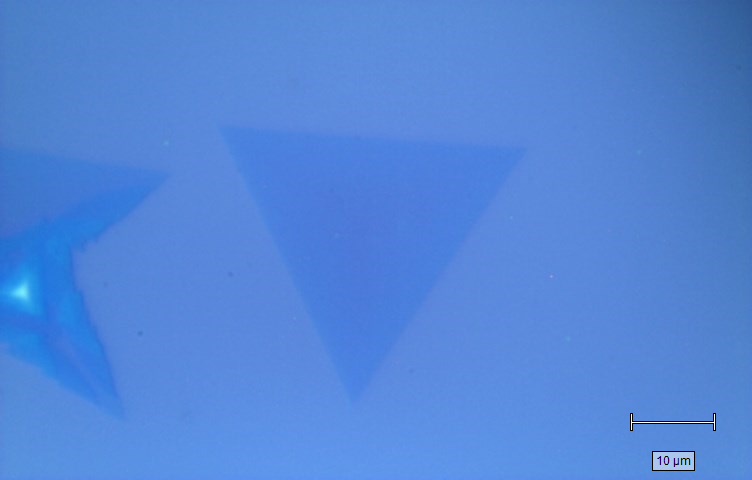
\includegraphics[scale=0.35]{WSe2/OMMap.png}
		\caption{A typical triangular monolayer flake}
		\label{fig:WSe2OMMap}
	\end{subfigure}
	\qquad
	\begin{subfigure}[b]{0.4\textwidth}
		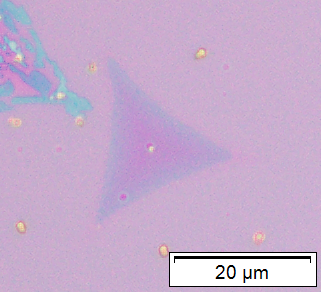
\includegraphics[scale=0.5]{WSe2/OMMap2.png}
		\caption{Triangular flake with visible strip of contrast along the edge}
		\label{fig:WSe2OMMap2}
	\end{subfigure}
	\caption{Optical micrographs of $WSe_2$ monolayer flakes}
\end{center}
\end{figure}

These flakes have been characterized by PL and Raman spectroscopy (Figure \ref{fig:WSe2PLRamanSpectra}. A typical PL and Raman spectrum can be seen in Figure \ref{fig:WSe2PLRamanSpectra}. The peak is centred at 1.65 eV which suggests a monolayer nature of the flake (as the direct band gap of monolayer is 1.65 eV) and the peak appears mostly symmetrical with FWHM of 66 meV. The symmetry of the peak and the fact it can be fitted with a single function, suggest a negligible contribution from trions in contrast to what we observed for $WS_2$  fakes. The Raman peak around 250 $cm^{-1}$ is a convolution of 2 peaks, an $E^1_{2g}$ and $A_{1g}$ vibrational modes, as already observed for bulk as well as exfoliated $WSe_2$.

\begin{figure}[H]
	\begin{center}
		\begin{subfigure}[b]{0.45\textwidth}
			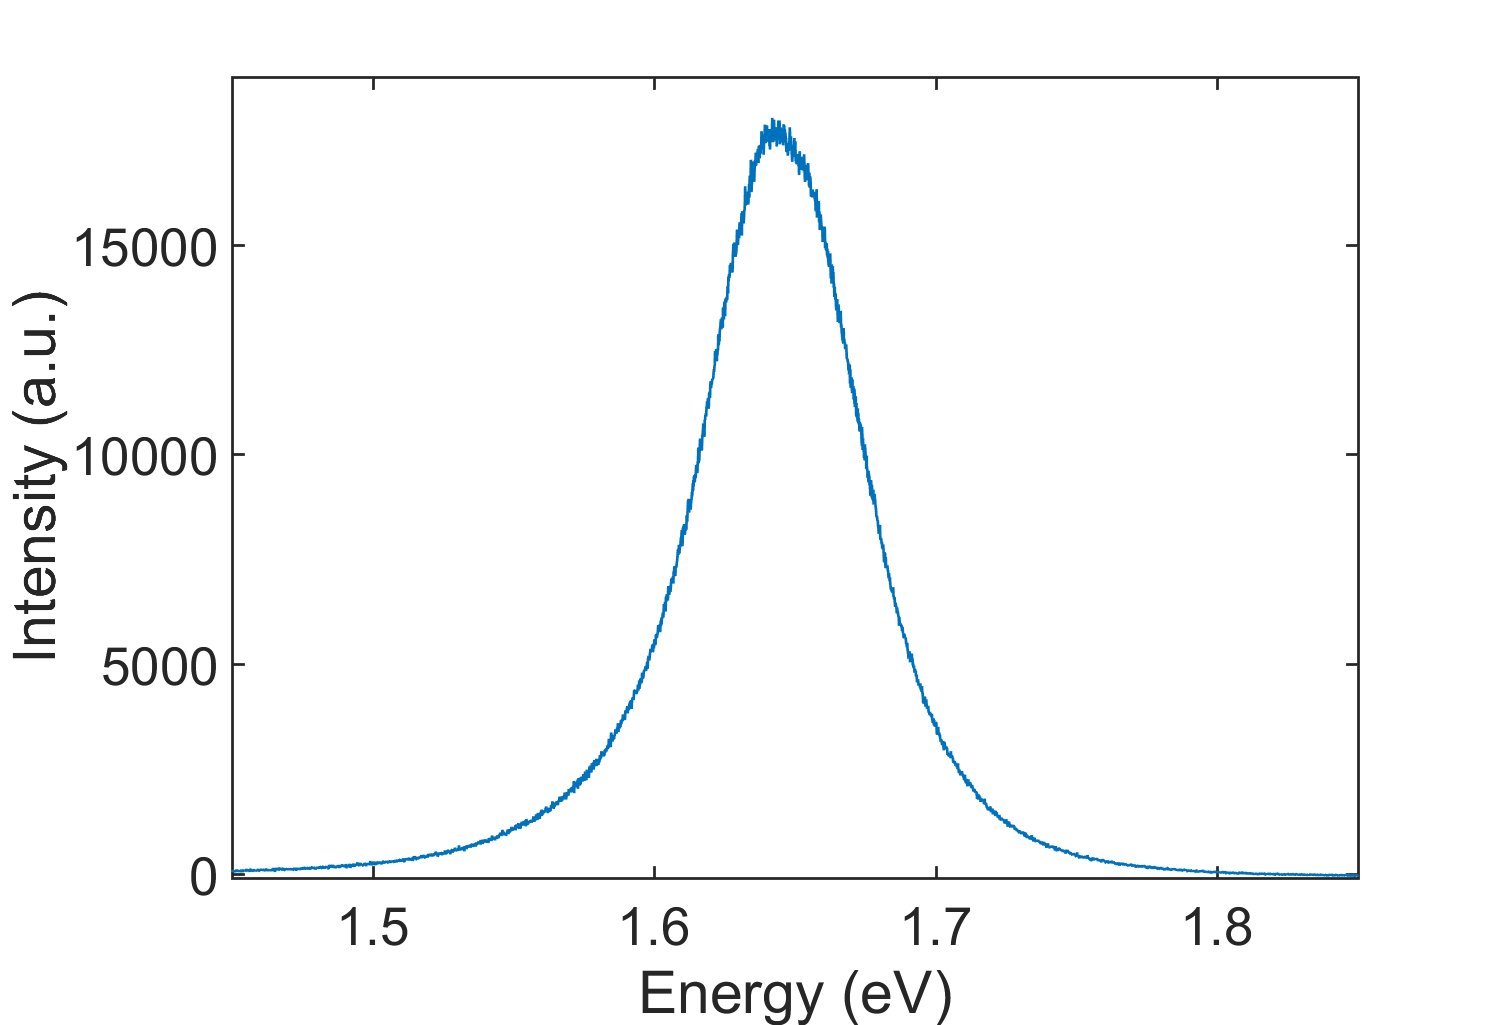
\includegraphics[width=\textwidth]{WSe2/PLSpectrum.png}
			\caption{Typical PL spectrum from monolayer $WSe_2$}
			\label{fig:WSe2PLSpectrum}
		\end{subfigure}
		\qquad
		\begin{subfigure}[b]{0.45\textwidth}
			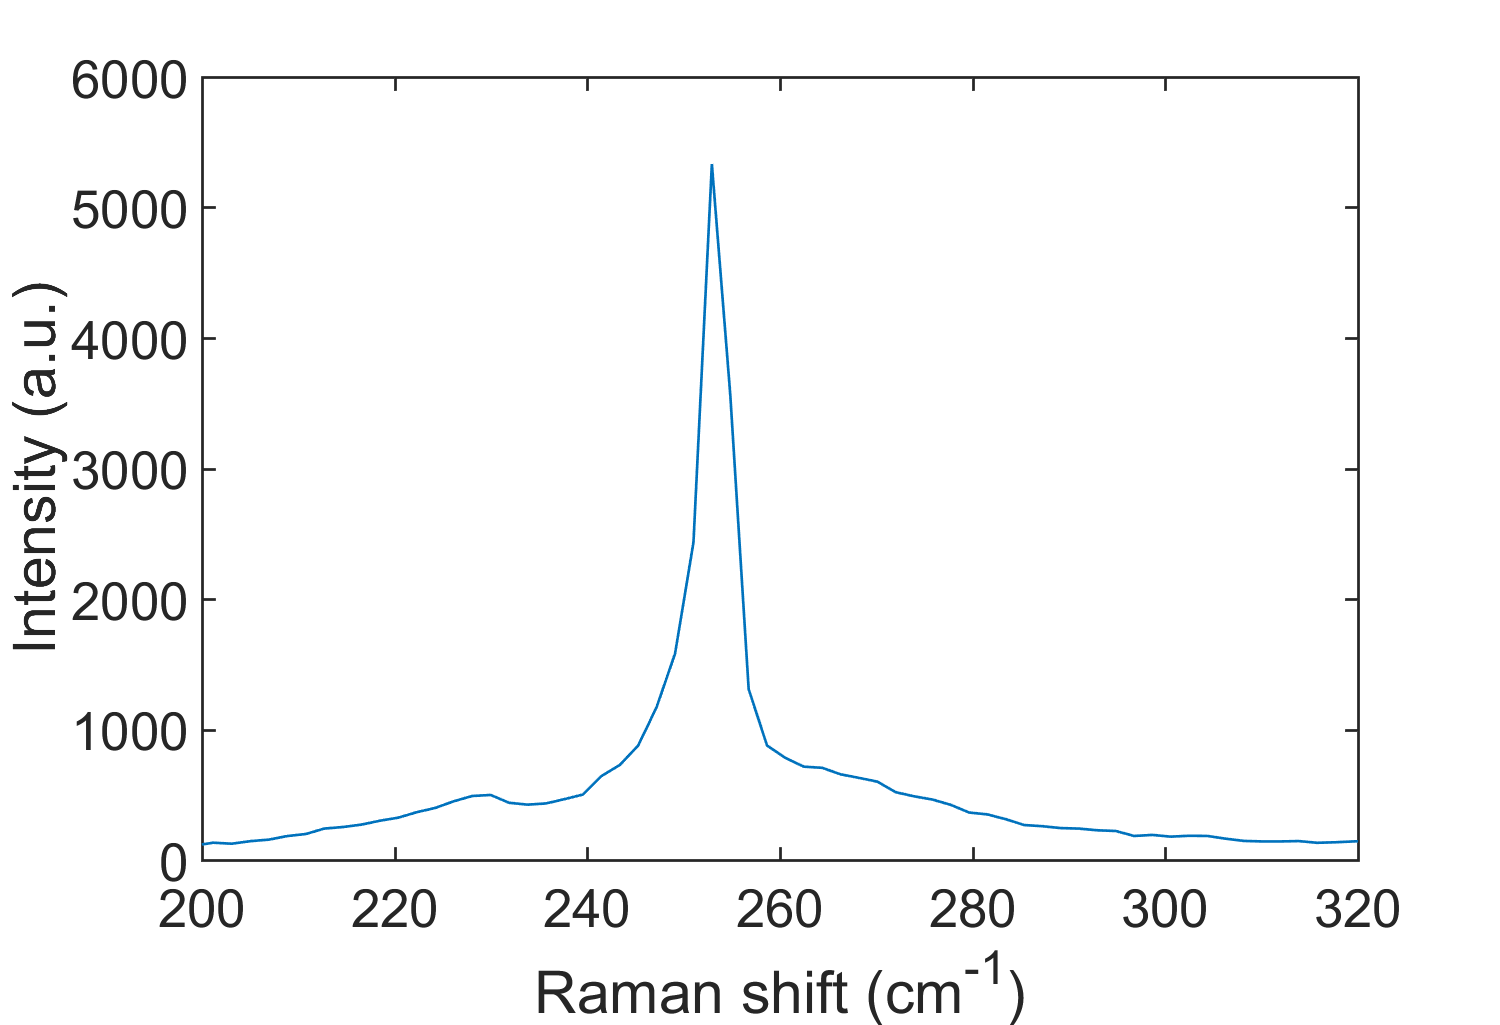
\includegraphics[width=\textwidth]{WSe2/RamanSpectrum.png}
			\caption{Typical Raman spectrum from monolayer $WSe_2$}
			\label{fig:WSe2RamanSpectrum}
		\end{subfigure}
		\caption{PL and Raman spectra from monolayer $WSe_2$}
		\label{fig:WSe2PLRamanSpectra}
	\end{center}
\end{figure}
	
\begin{figure}[H]
	\begin{center}
		\begin{subfigure}[b]{0.45\textwidth}
			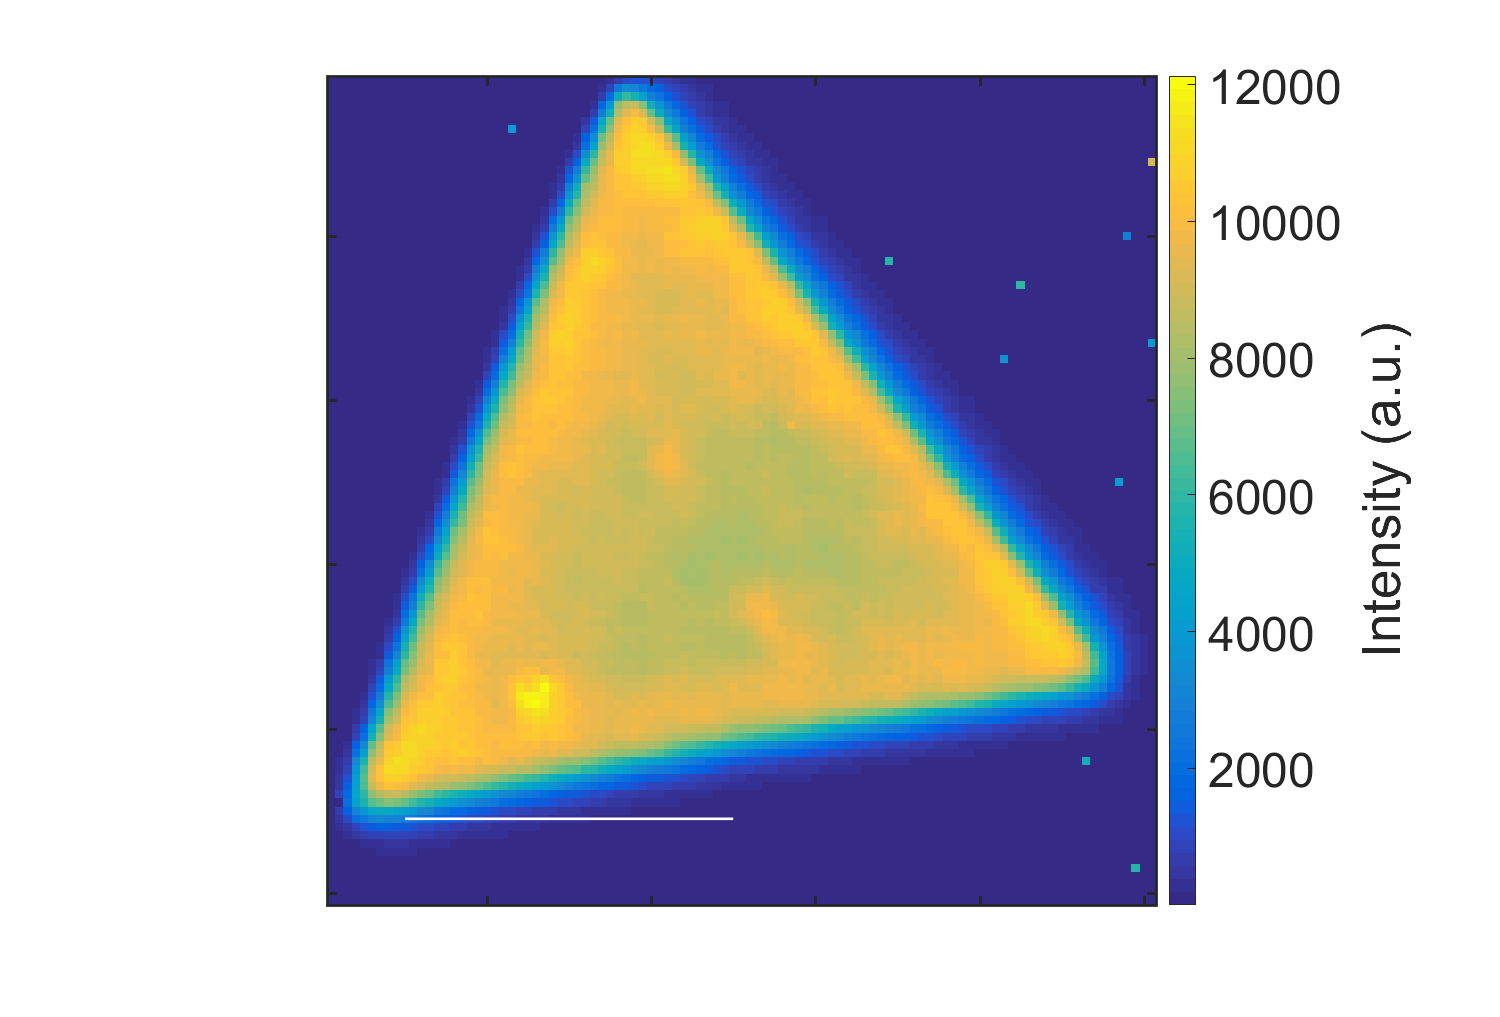
\includegraphics[width=\textwidth]{WSe2/PLIntensity.png}
			\caption{PL intensity}
			\label{fig:WSe2PLIntensityMap}
		\end{subfigure}
		\qquad
		\begin{subfigure}[b]{0.45\textwidth}
			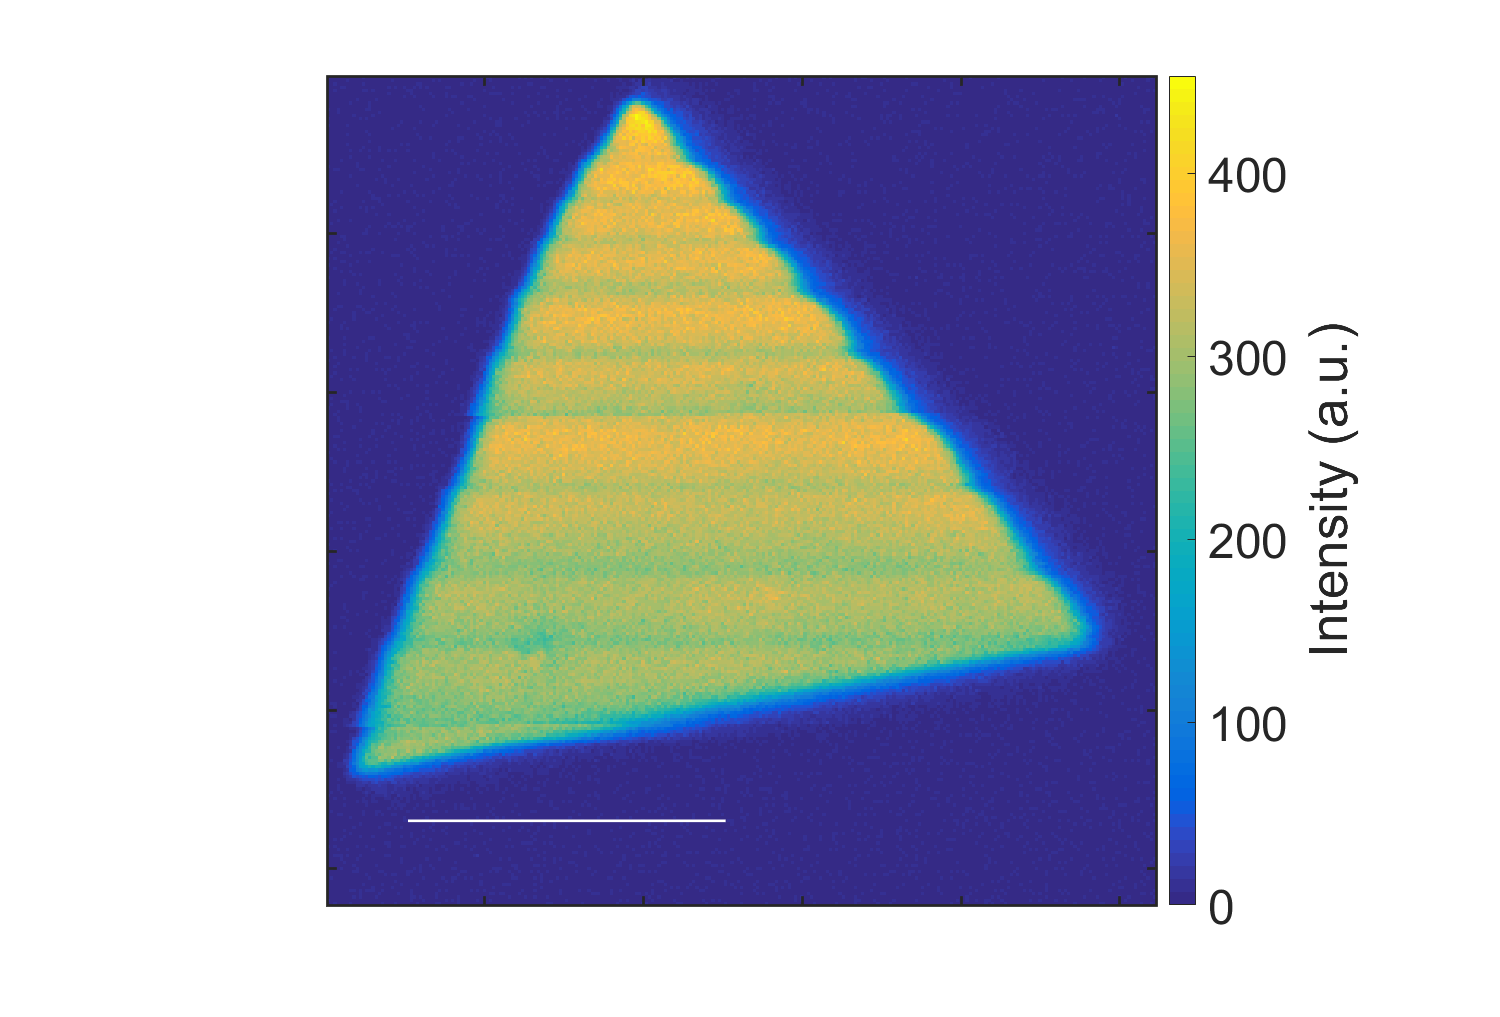
\includegraphics[width=\textwidth]{WSe2/RamanEIntensity.png}
			\caption{Raman $E^1_{2g}$ intensity}
			\label{fig:WSe2RamanIntensityMap}
		\end{subfigure}
		\caption{PL intensity and Raman $E^1_{2g}$ intensity maps}
	\end{center}
\end{figure}

A typical map of PL intensity of a $WSe_2$ sample can be seen in Figure \ref{fig:WSe2PLIntensityMap}. Compared to the $WS_2$ samples grown using the same procedure the PL intensity is much more homogeneous throughout the flake. In particular it does not exhibit the trisecting pattern as seen in $WS_2$ samples e.g. Figure \ref{fig:WSe2PLIntensityMap}. Similarly the Raman $E^1_{2g}$ peak intensity map as seen in Figure \ref{fig:WSe2RamanIntensityMap} also does not show the same pattern of trisecting lines. Due to technical issues with the spectrometer the map in Figure \ref{fig:WSe2RamanIntensityMap} shows periodically repeating horizontal lines of lower intensity.
	
\begin{figure}[!h]
	\begin{center}
		\begin{subfigure}[b]{0.45\textwidth}
			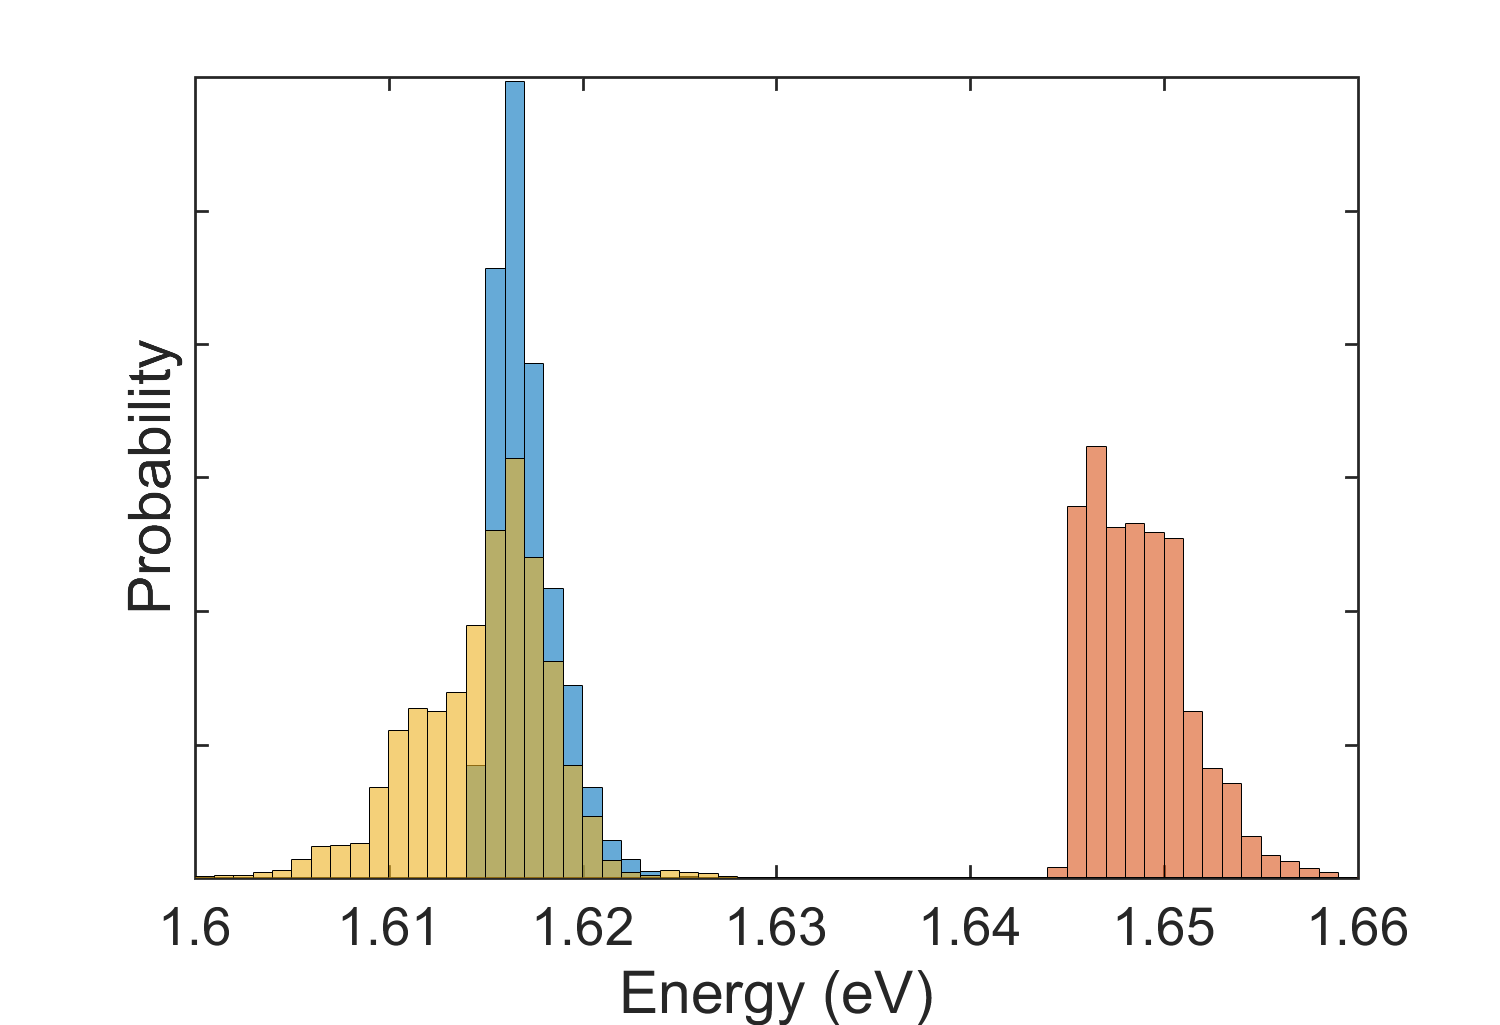
\includegraphics[width=\textwidth]{WSe2/WSe2PositionHistograms.png}
			\caption{WSe2 PL peak positions histograms}
			\label{fig:WSe2PLPositionHistograms}
		\end{subfigure}
		\qquad
		\begin{subfigure}[b]{0.45\textwidth}
			\includegraphics[width=\textwidth]{WSe2/Wse2WidthHistograms.png}
			\caption{WSe2 PL peak positions histograms}
			\label{fig:WSe2PLWidthHistograms}
		\end{subfigure}
		\caption{Comparison of PL peak positions and widths in different $WSe_2$ samples. Different colour correspond to separate growths.}
		\label{fig:WSe2PLHistograms}
	\end{center}
\end{figure}

A comparison of PL peak positions and widths between different samples of $WSe_2$, all grown using the same conditions, can be seen in Figure \ref{fig:WSe2PLHistograms}.

\begin{figure}[H]
	\begin{center}
		\begin{subfigure}[b]{0.45\textwidth}
			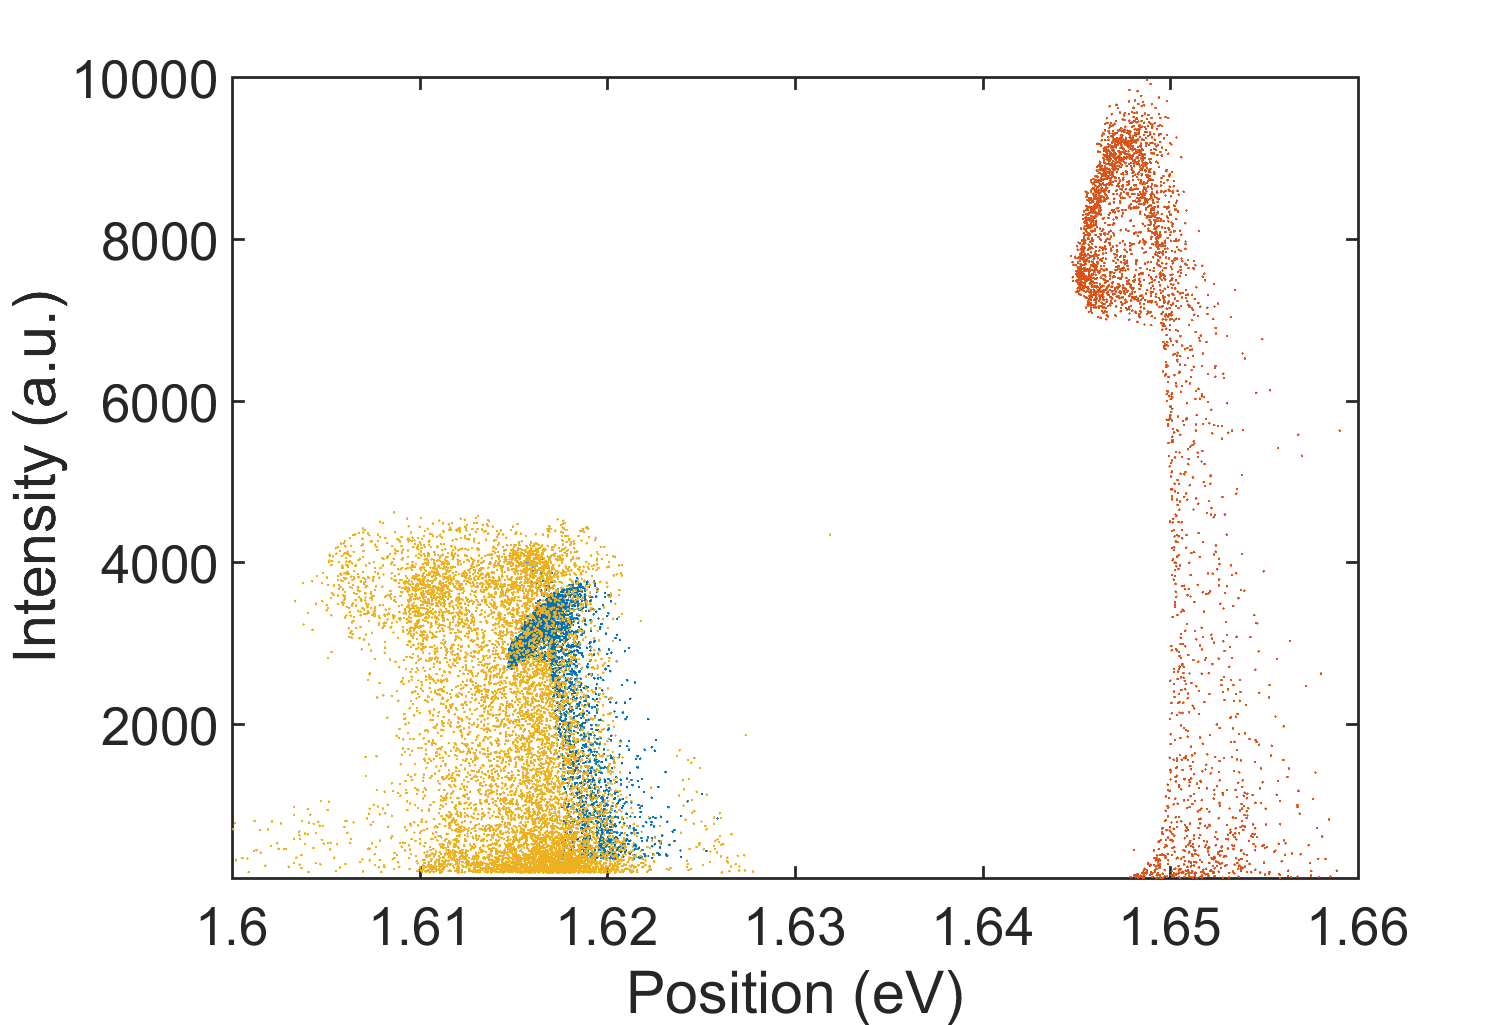
\includegraphics[width=\textwidth]{WSe2/WSe2PositionIntensityScatterComparison.png}
			\caption{Intensity vs position}
			\label{fig:WSe2PositionIntensityScatterComparison}
		\end{subfigure}
		\qquad
		\begin{subfigure}[b]{0.45\textwidth}
			\includegraphics[width=\textwidth]{WSe2/Wse2PositionWidthScatterComparison.png}
			\caption{Width vs position}
			\label{fig:WSe2PositionWidthScatterComparison}
		\end{subfigure}
		\caption{PL peak parameters distribution}
		\label{fig:WSe2ScatterComparison}
	\end{center}
\end{figure}

By plotting the intensity and width of the PL peaks against the peak position as seen in Figure \ref{fig:WSe2ScatterComparison} certain patterns can be observed. The intensity is mostly grouped around maximum values and relatively narrowly spread across the position spectrum. One of the growths (in red) shows much more even distribution of intensity across the position, which combined with the wide distribution of positions results in a much more inhomogeneous sample. The PL FWHM and positions are generally well grouped with flakes with smaller FWHM having more narrow distribution than those with greater width. Also the flake with greater average PL peak position shows a smaller peak width. Overall there is no obvious relation between position and width.

%% Raman

For most of the TMDCs Raman can be used to identify the number of layers or strain within the layer. However in the case of $WSe_2$ the position of the $E^1_{2g}$ and $A_{1g}$ largely overlaps and therefore it is difficult to accurately determine the difference in their position. Because of that this method of identifying the number of layers cannot be employed easily. It is however still possible to examine the strain within the layers by noting the shift of the $E^1_{2g}$ peak. A Raman $E^1_{2g}$ peak position distribution from a representative sample can be seen in Figure \ref{fig:WSe2RamanPositionHistogram1}. The strain can be then determined from the mean position of $250.7 \pm 0.01$ $cm^{-1}$ to be 2.44 {\%} \cite{Dadgar2018}.

\begin{figure}[H]
	\begin{center}
		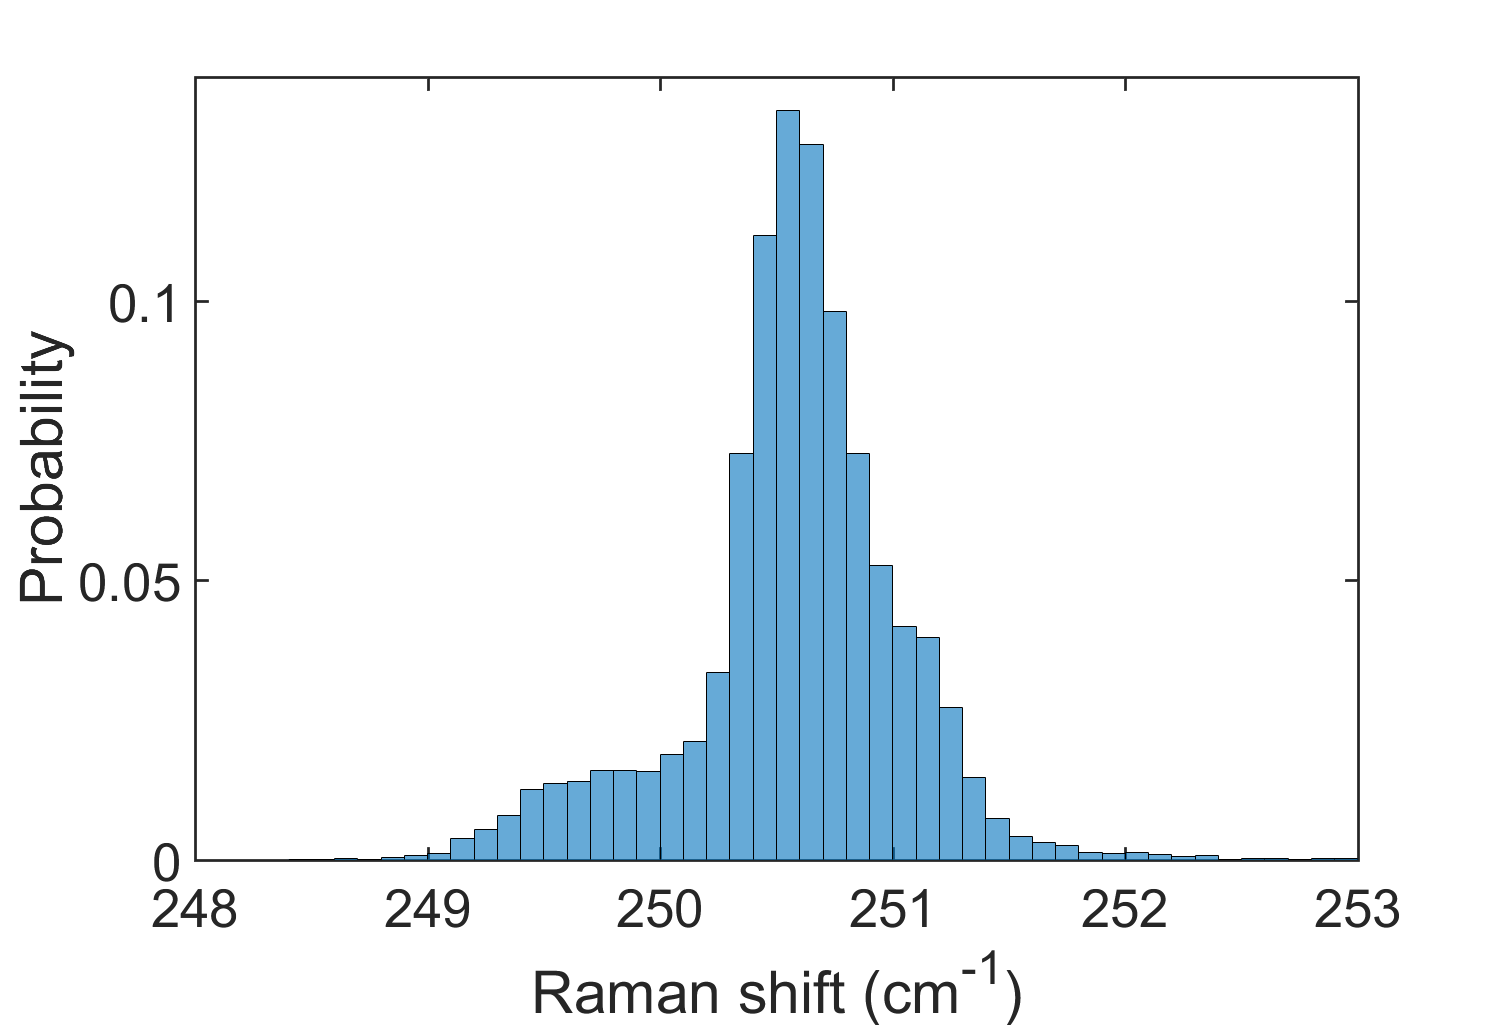
\includegraphics[scale=0.35]{WSe2/WSe2RamanPositionHistogram1.png}
		\caption{Histogram of Raman $E^1_{2g}$ peak position from monolayer $WSe_2$}
		\label{fig:WSe2RamanPositionHistogram1}
	\end{center}
\end{figure}

\begin{figure}[!h]
	\begin{center}
		\begin{subfigure}[b]{0.4\textwidth}
			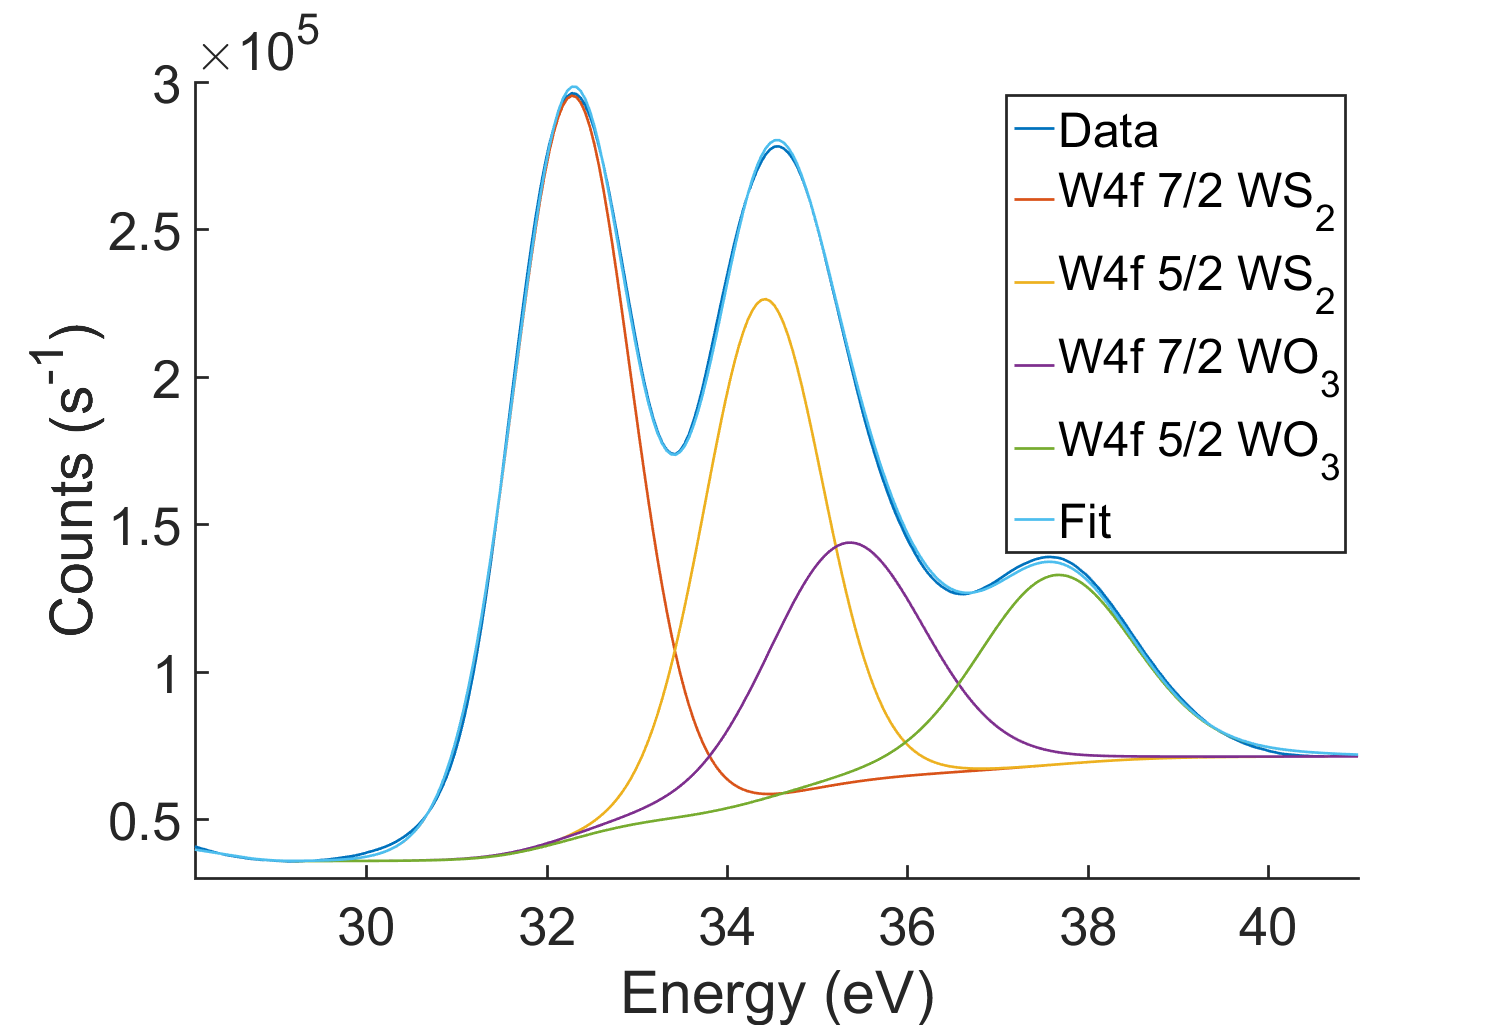
\includegraphics[width=\textwidth]{WSe2/XPSW4fThin.png}
			\caption{Thin flakes}
			\label{fig:WSe2XPSThinW}
		\end{subfigure}
		\qquad
		\begin{subfigure}[b]{0.4\textwidth}
			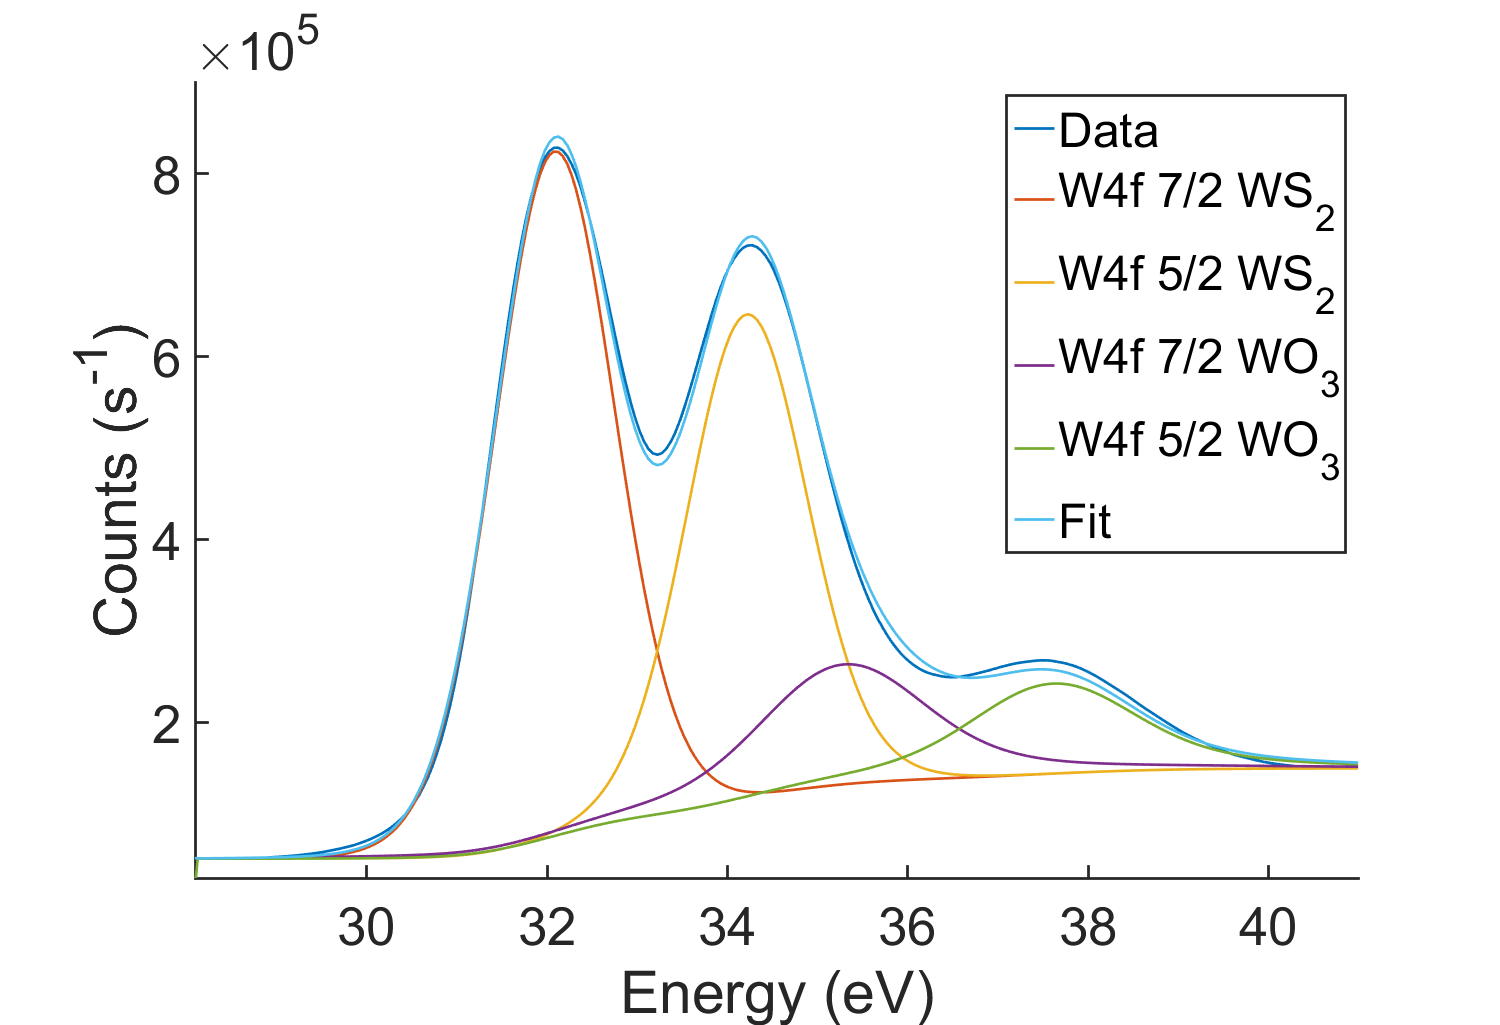
\includegraphics[width=\textwidth]{WSe2/XPSW4fThick.png}
			\caption{Thick flakes}
			\label{fig:WSe2XPSThickW}
		\end{subfigure}
		
		\begin{subfigure}[b]{0.4\textwidth}
			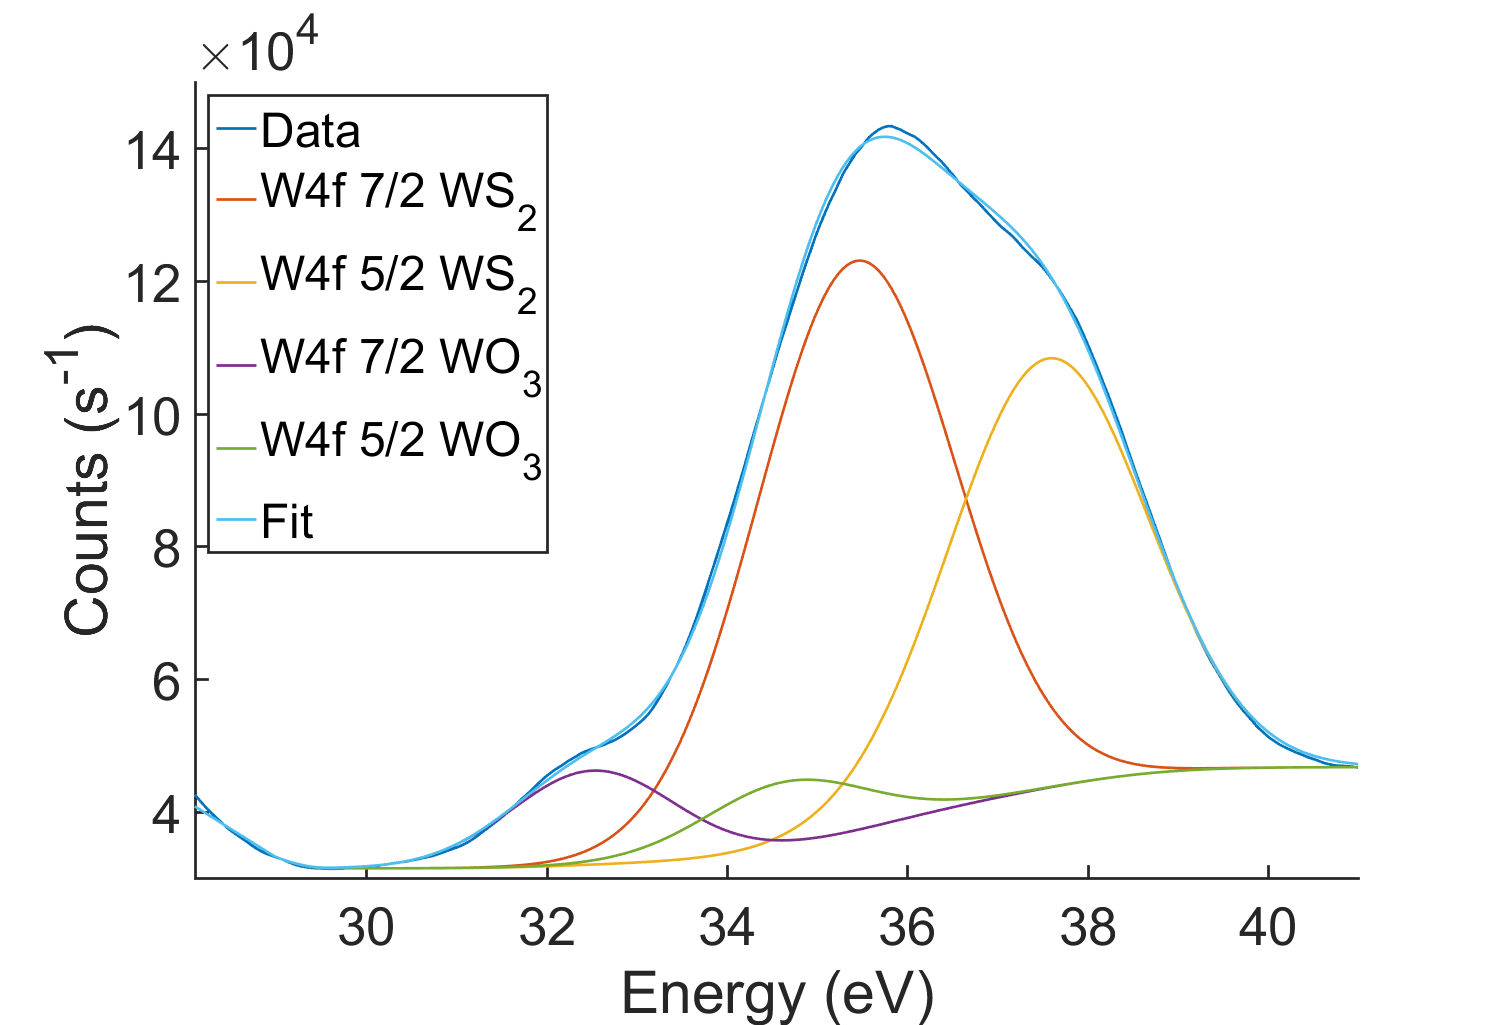
\includegraphics[width=\textwidth]{WSe2/XPSW4fRef.png}
			\caption{Empty area}
			\label{fig:WSe2XPSRefW}
		\end{subfigure}
		\caption{XPS spectra of W4f peaks in different areas of the sample}
		\label{fig:WSe2XPSW}
	\end{center}
\end{figure}

\begin{figure}[H]
	\begin{center}
		\begin{subfigure}[b]{0.4\textwidth}
			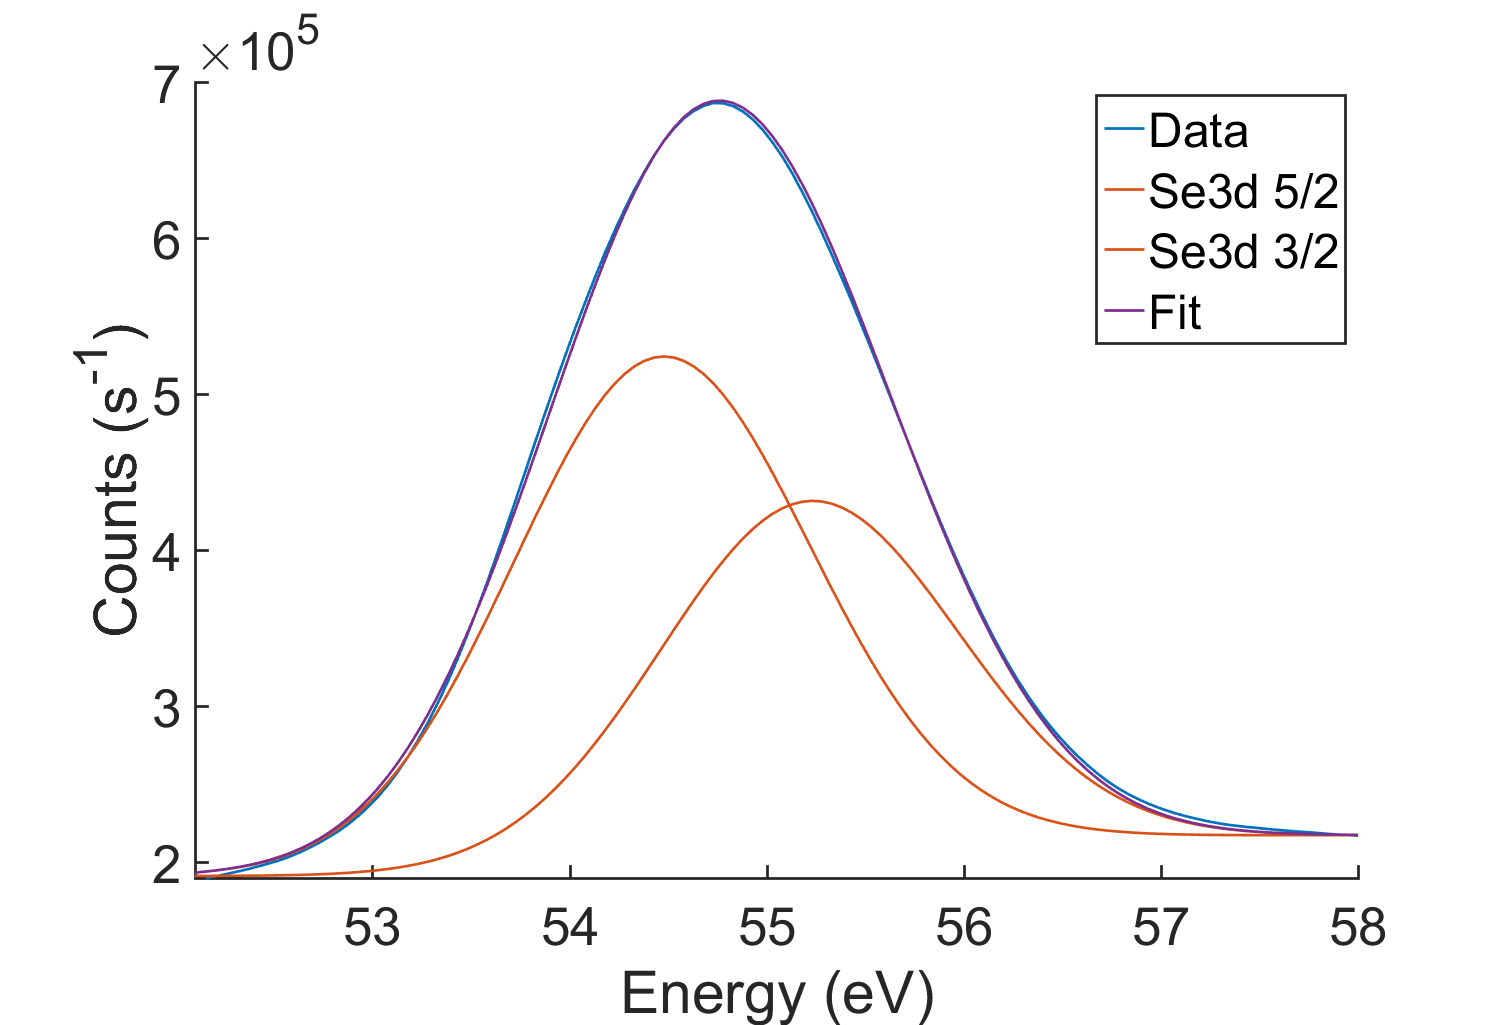
\includegraphics[width=\textwidth]{WSe2/XPSSe3dThin.png}
			\caption{Thin flakes}
			\label{fig:WSe2XPSThinSe}
		\end{subfigure}
		\qquad
		\begin{subfigure}[b]{0.4\textwidth}
			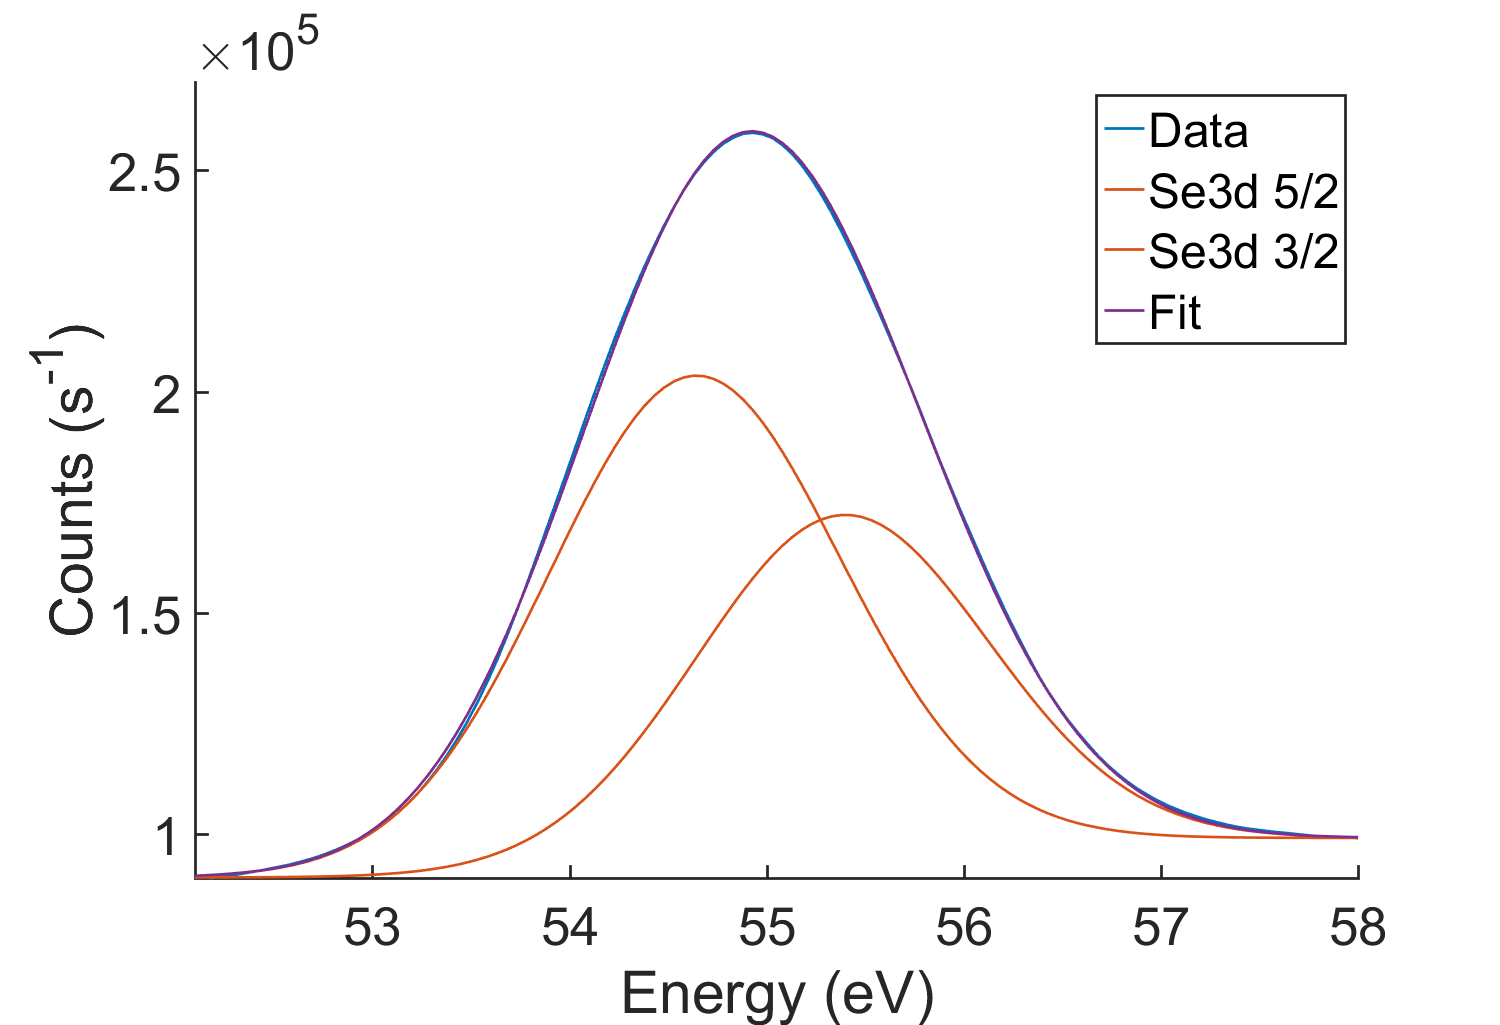
\includegraphics[width=\textwidth]{WSe2/XPSSe3dThick.png}
			\caption{Thick flakes}
			\label{fig:WSe2XPSThickSe}
		\end{subfigure}
		
		\begin{subfigure}[b]{0.4\textwidth}
			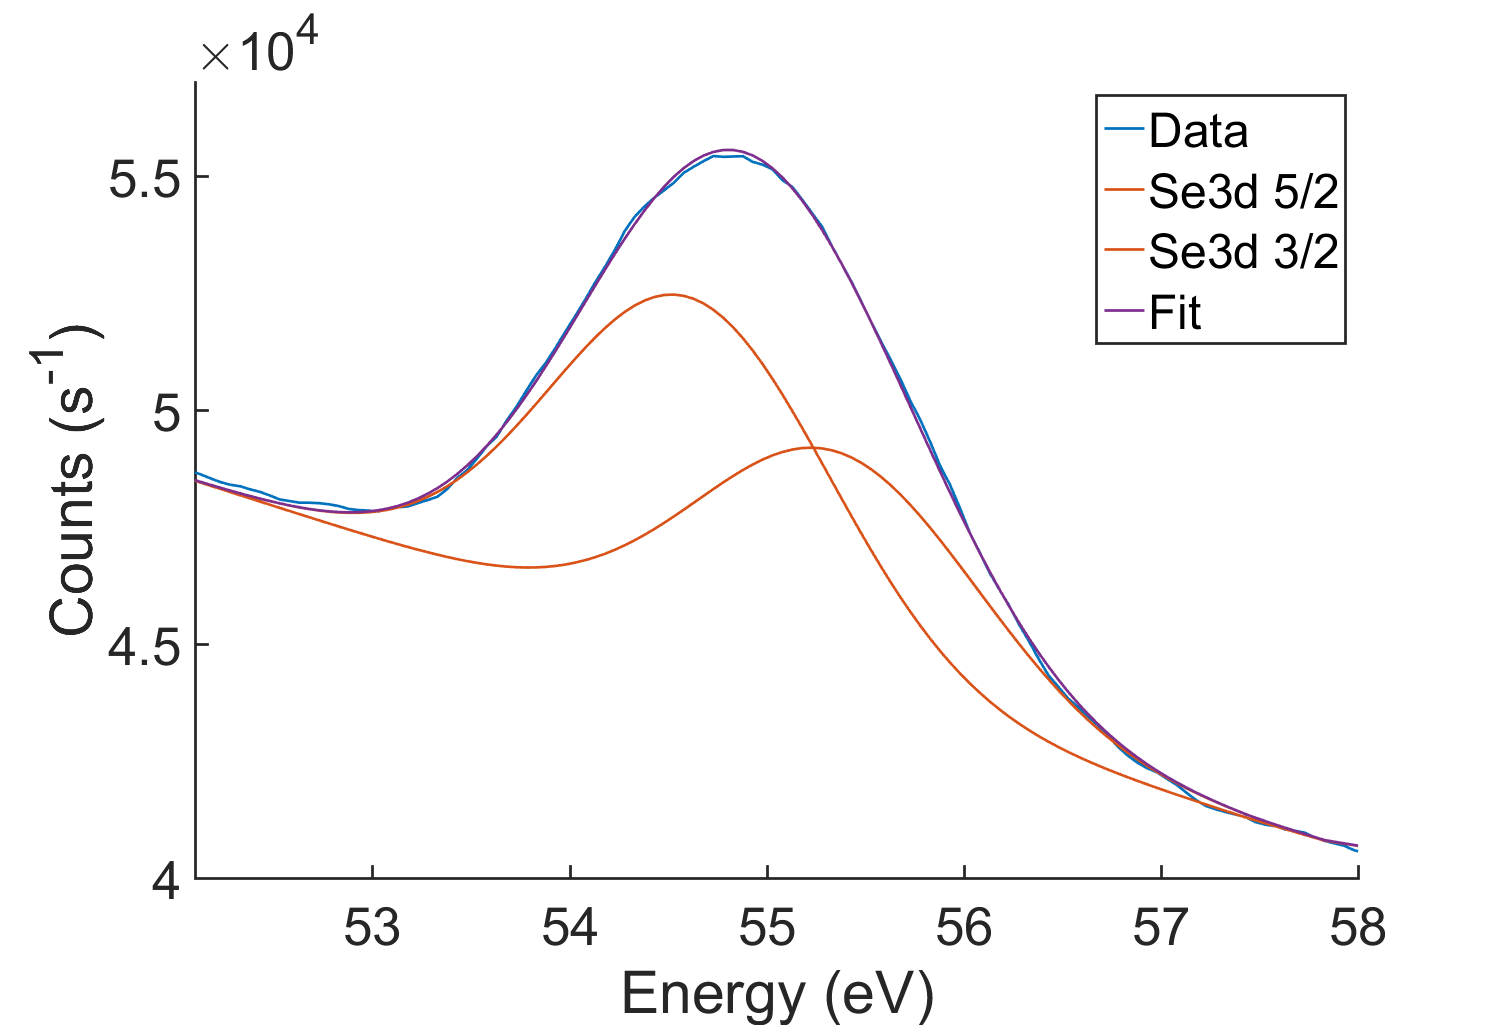
\includegraphics[width=\textwidth]{WSe2/XPSSe3dRef.png}
			\caption{Empty area}
			\label{fig:WSe2XPSRefSe}
		\end{subfigure}
		\caption{XPS spectra of Se3d peaks in different areas of the sample}
		\label{fig:WSe2XPSSe}
	\end{center}
\end{figure}

\begin{figure}[!h]
	\begin{center}
		\begin{subfigure}[b]{0.4\textwidth}
			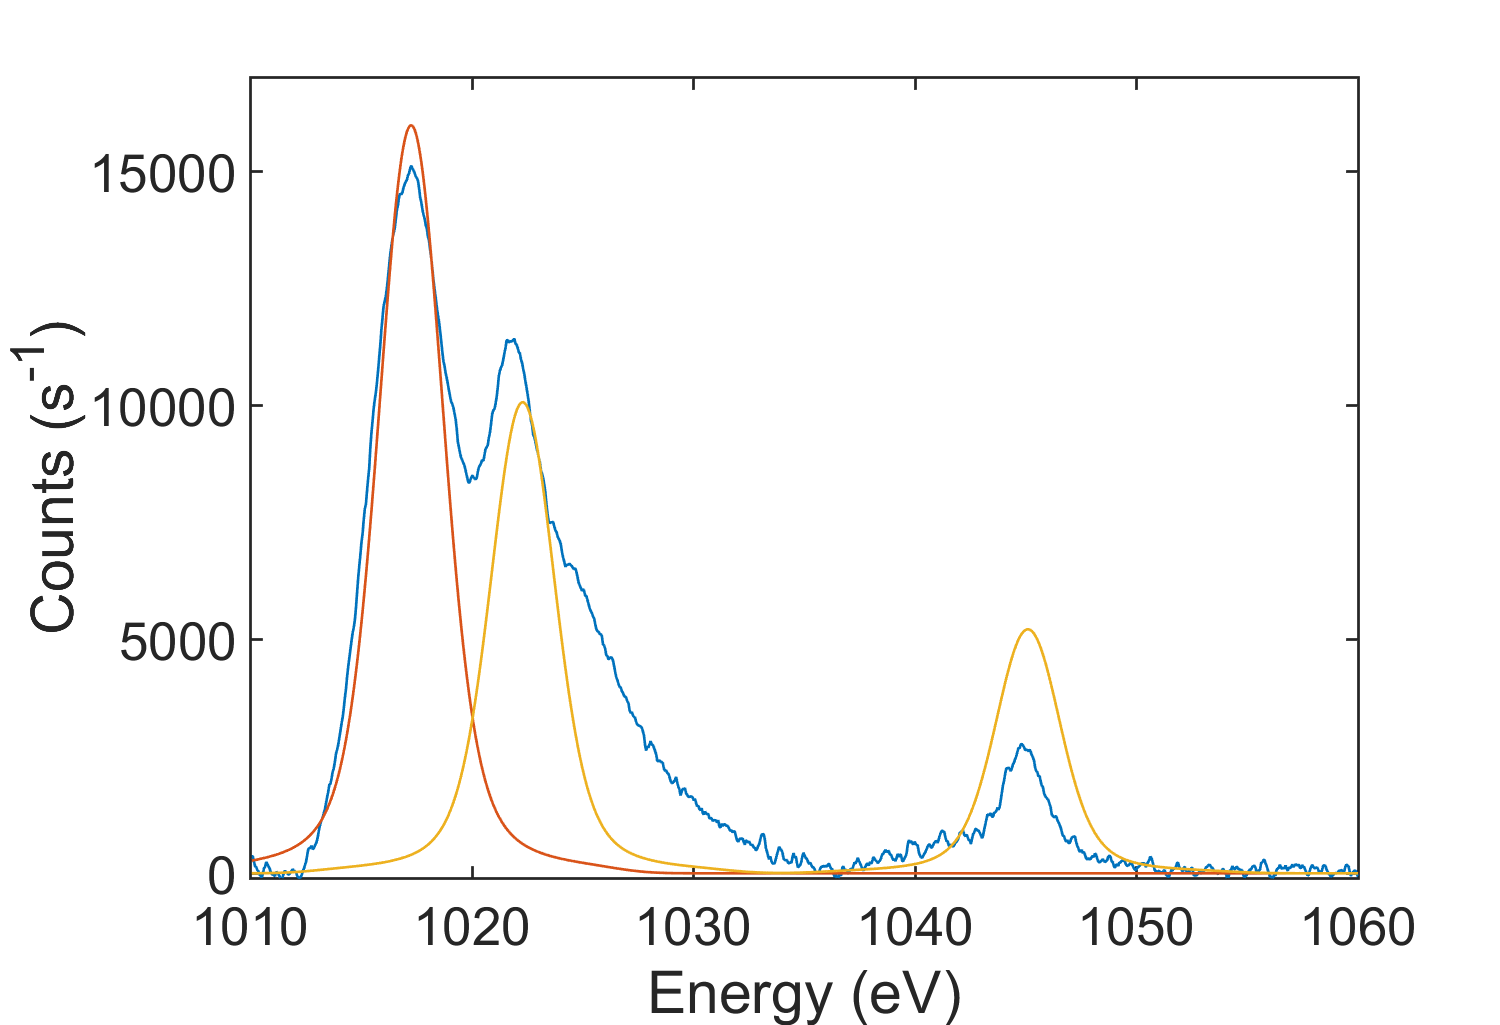
\includegraphics[width=\textwidth]{WSe2/WSe2XPSThinZn.png}
			\caption{Thin flakes}
			\label{fig:WSe2XPSThinZn}
		\end{subfigure}
		\qquad
		\begin{subfigure}[b]{0.4\textwidth}
			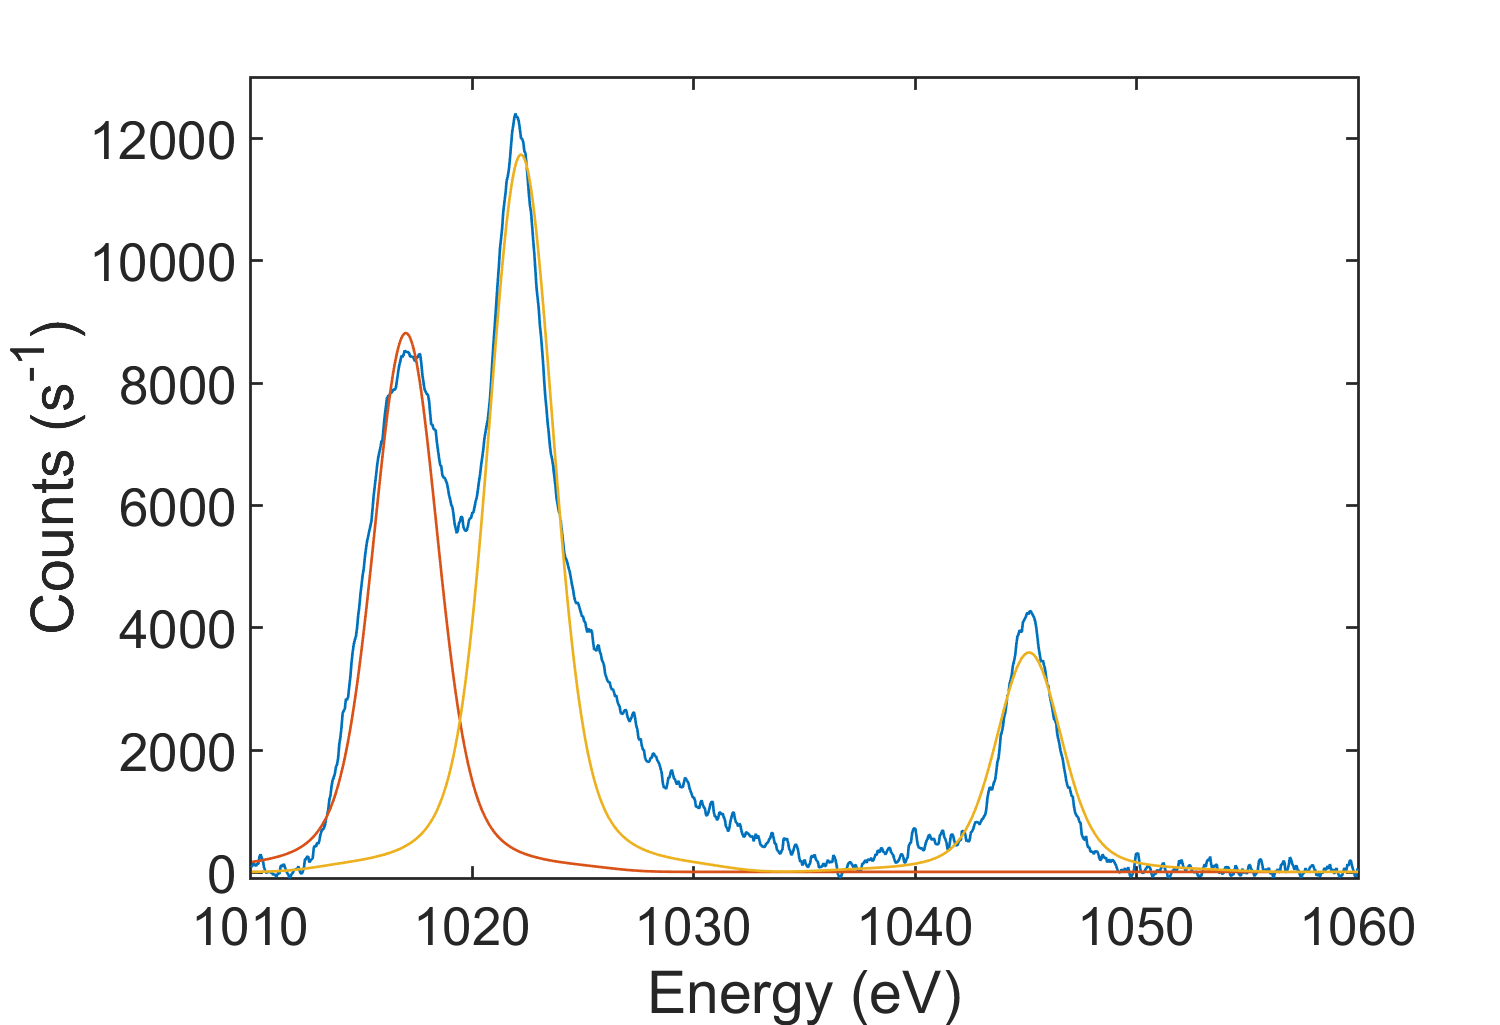
\includegraphics[width=\textwidth]{WSe2/WSe2XPSThickZn.png}
			\caption{Thick flakes}
			\label{fig:WSe2XPSThickZn}
		\end{subfigure}
		
		\begin{subfigure}[b]{0.4\textwidth}
			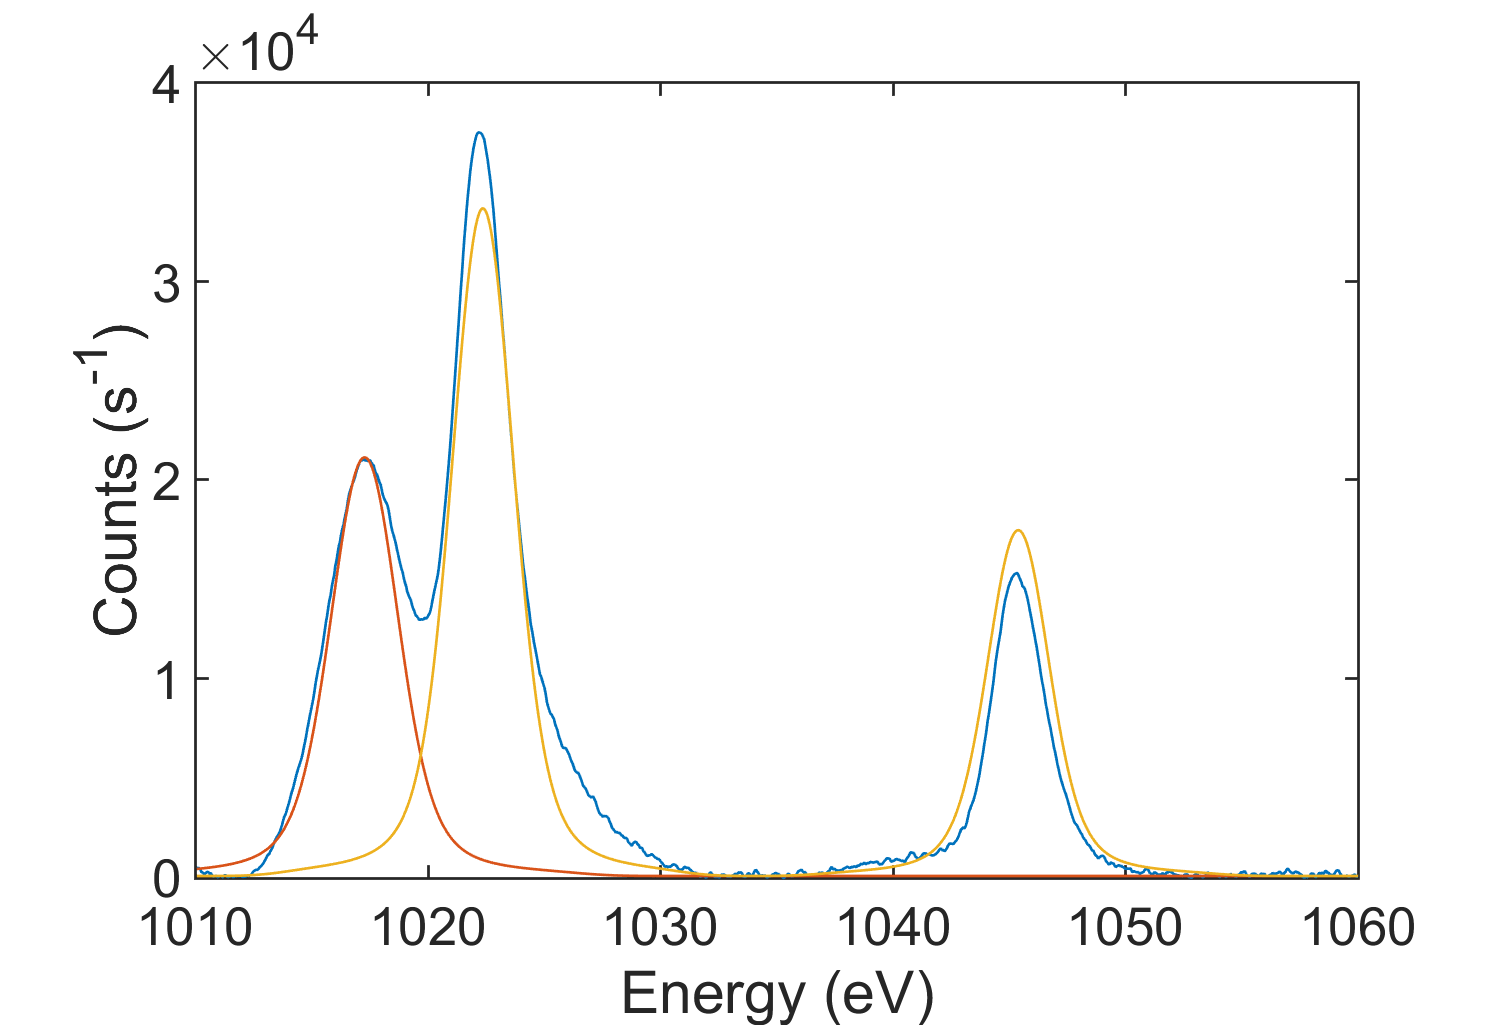
\includegraphics[width=\textwidth]{WSe2/WSe2XPSRefZn.png}
			\caption{Empty area}
			\label{fig:WSe2XPSRefZn}
		\end{subfigure}
		\caption{XPS spectra of Zn2p peaks in different areas of the sample}
		\label{fig:WSe2XPSZn}
	\end{center}
\end{figure}

The sample has been further characterised with XPS. Three areas were selected for measurements, one with thin, mono or double layer $WSe_2$, one with thick bulk $WSe_2$ and one with no visible $WSe_2$ flakes. The Figure \ref{fig:WSe2XPSW} shows W4f core levels measured in those spots. The first area (Figure \ref{fig:WSe2XPSThinW}), with thin flake shows one doublet at 32.08 eV and 34.23 eV and a second doublet at 35.33 eV and 37.68 eV. The first doublet corresponds to $WSe_2$ while the second one can be attributed to $WO_3$. Since the spot size in the measurement covers both the flake as well as some surrounding substrate it is possible that the $WO_3$ is located outside of the flake. Furthermore the background indicates that the emission from $WSe_2$ came from the surface and therefore the $WSe_2$ flake is not contaminated with $WO_3$. 
The second area with thicker flakes (Figure \ref{fig:WSe2XPSThickW}) shows similarly two doublets: one at 32.28 eV and 34.43 eV and a second one at 35.38 eV and 37.63 eV. Similarly to the area with  the thin flake we can ascribe the former to the $WSe_2$ and the latter to $WO_3$. There is a small shift of 0.2 eV between $WSe_2$ from the thin flake and $WSe_2$ from the thick flake. It is possible that XPS is sensitive to the number of layers in $WSe_2$ and TMDCs in general since it is known that number of layers does modify the electronic structure of the material \cite{ElectronicsAndOptoelectronicsOfTwo-dimensionalTransitionMetalDichalcogenides}. The $WO_3$ is found to be at the same position in both areas. The $WO_3$ peak is also relatively weaker in the area with the thick flake than in the area with thin flake which could be a result of the thick flake having larger surface area than the thin flake and smaller presence of $WO_3$ around the flake. 
Additionally an empty area (Figure \ref{fig:WSe2XPSRefW}) with no visible flakes has been measured. Similarly two doublets, one at 32.58 eV and 34.73 eV and a second one at 35.48 eV and 37.58 eV have been fitted and their presence can be again explained by presence of $WSe_2$ and $WO_3$. The $WSe_2$ peak is shifted in relation to that from the thin flake by 0.5 eV which could indicate presence of a highly defective $WS_2$ or very small amounts of very bulk $WS_2$. The $WS_2$ peak is also much weaker than that of the $WO_3$ which is expected since there is no visible $WS_2$. This result suggesting presence of residues of tungsten oxide species across the whole substrate and thus also possibly across the grown flakes of $WSe_2$. This result corroborates the evidence of chemical purity of $WSe_2$.

We can also look at Se3d core levels measured at the same locations. As seen in Figure \ref{fig:WSe2XPSThinSe}, taken from an area with the thin flake, we can fit it with one doublet corresponding to the presence of $WSe_2$ at 54.48 eV and 55.23 eV. Similarly in Figure \ref{fig:WSe2XPSThickSe} we can see Se3d peaks taken from area with the thick flake and can fit it with a doublet at 54.63 eV and 55.38 eV which also corresponds to the $WSe_2$. Similar to the W4f levels there is a shift of 0.15 eV between those two flakes which can be explained by their thickness which changes the electronic structure. The Se3d levels measured in the reference empty area also can be fitted with a doublet at 54.53 eV and 55.33 eV which can be attributed to $WSe_2$. Similarly there is a shift of 0.05 eV from the peak associated with the thin flake, which is much smaller than the W4f peak shift. The Se3d peak from the empty area is about a magnitude weaker than that from either the thin or thick flake which is expected as no visible flake was observed. It does however indicate a non insignificant presence of $WSe_2$, perhaps in the form of nuclei that never grew into proper flakes or flakes that shrunk or became etched and are highly defective and thinner than monolayer. The Se3d from the empty area also exhibits a steep background which indicates that the Se is covered with some layer, perhaps that of $WO_3$. 

Finally the Zn2p levels were measured across the same areas. As seen in Figure \ref{fig:WSe2XPSThinZn} a doublet can be identified at 1022.02 eV and 1045.11 eV together with a single peak at 1017.33 eV taken from a thin flake. Similarly in Figure \ref{fig:WSe2XPSThickZn} the doublet is located at 1022.23 eV and 1045.16 eV and a single peak at 1017.03 eV. The reference area shows a doublet at 1045.39 eV and 1022.38 eV and a single peak at 1017.29 eV. It seems therefore that the peak position of the Zn2p doublet does not changes significantly from the empty reference area and the thin or thick flake. The peak intensity in the empty area is also much greater than that of the peak in the area with thin or thick flakes. It suggests then that the Zn that was used in the synthesis is therefore located mostly on a substrate and not on the $WSe_2$ flakes.

\begin{center}
\begin{table}[H]
\caption{$WSe_2$ W 4f and Se 3d peak position dependance on number of layers}
\label{tab:WSe2XPSTableComparison}
\end{table}
\end{center}
\begin{center}
\begin{tabular}{c|cc}
		& Thin ($<$3 layers) 	& Thick ($\sim$6 layers)\\ \hline
W 4f7	& 32.08 eV				& 32.28 eV				\\ 
W 4f5	& 34.23 eV				& 34.43 eV				\\
Se 3d5 	& 54.48 eV				& 54.63 eV				\\
Se 3d3  & 55.23 eV				& 55.38 eV				
\end{tabular}
\end{center}

As seen in Table \ref{tab:WSe2XPSTableComparison} the peak positions of W 4f and Se 3d taken from $WSe_2$ thin and thick flakes can be compared. The thick flake can be considered to be equivalent to a bulk form. There is a consistent shift of about 0.2 eV for all of those peaks.

\subsection{Colloidal synthesis of 1T' and 2H $WSe_2$}

The sample was characterised using TEM as seen in Figure \ref{fig:1T'TEMMaps}. The TEM images show well defined flower shaped nanostructures with the average diameter of 200 nm. The petals stem from the central point and thin down towards the edges down to single layer. The single petals appear to be of 1T' phase while each petal is a single crystal. Additionally the structural parameters a = 5.76 \r{A} and b = 3.30 \r{A} have been identified. Reciprocal lattice created by FFT from high resolution TEM image from a single petal is rectangular and corresponding to monoclinic phase of $WSe_2$.

\begin{figure}[H]
	\begin{center}
		\begin{subfigure}[b]{0.4\textwidth}
			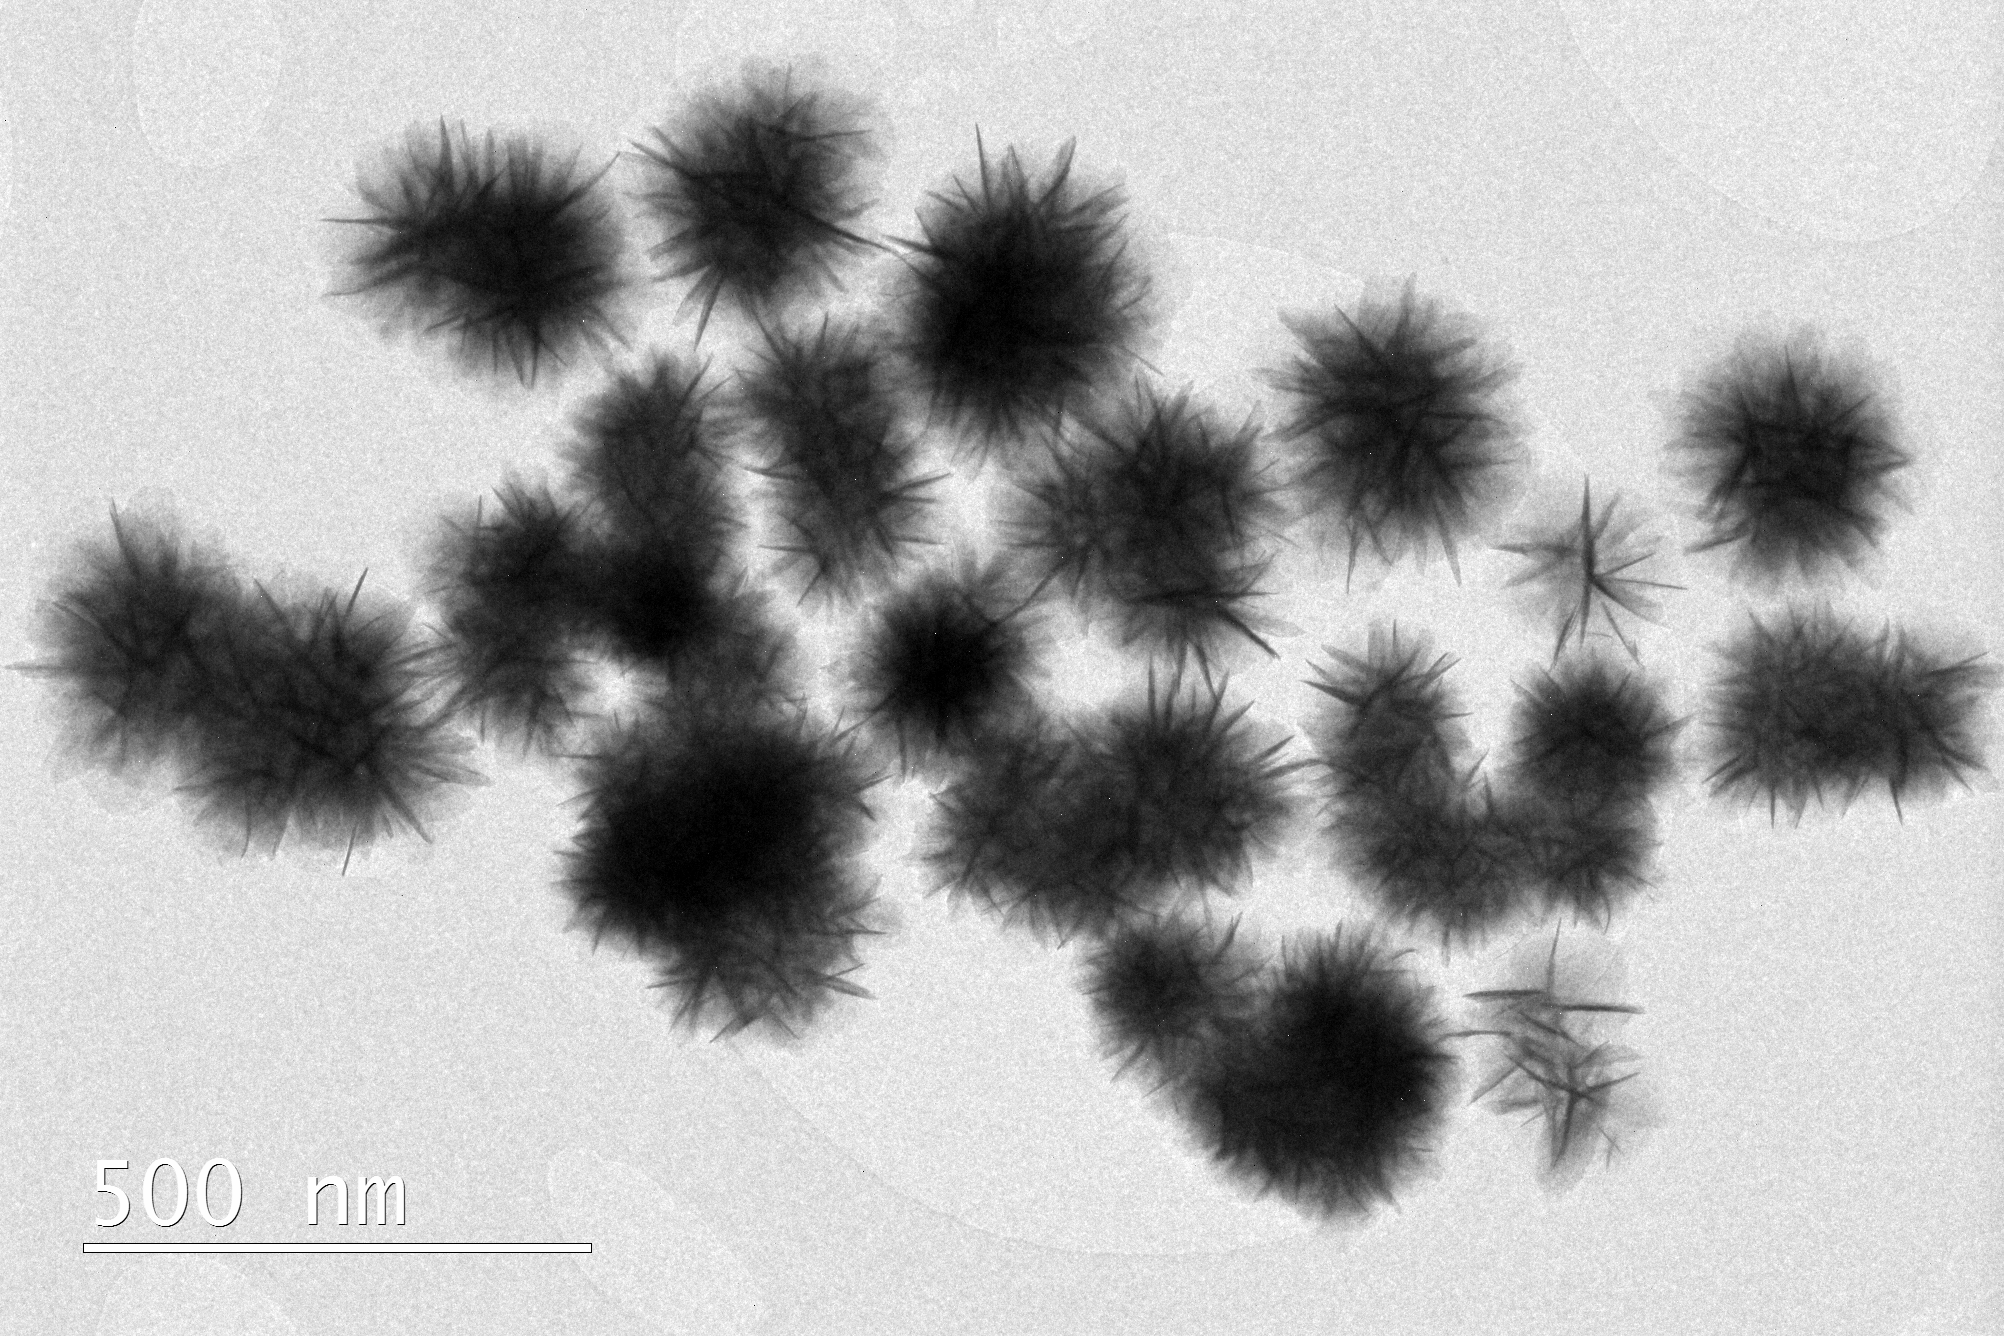
\includegraphics[width=\textwidth]{1T'/TEMImage.png}
			\caption{TEM image of as grown 1T' $WSe_2$ flakes.}
			\label{fig:1T'TEMImage}
		\end{subfigure}
		\qquad
		\begin{subfigure}[b]{0.4\textwidth}
			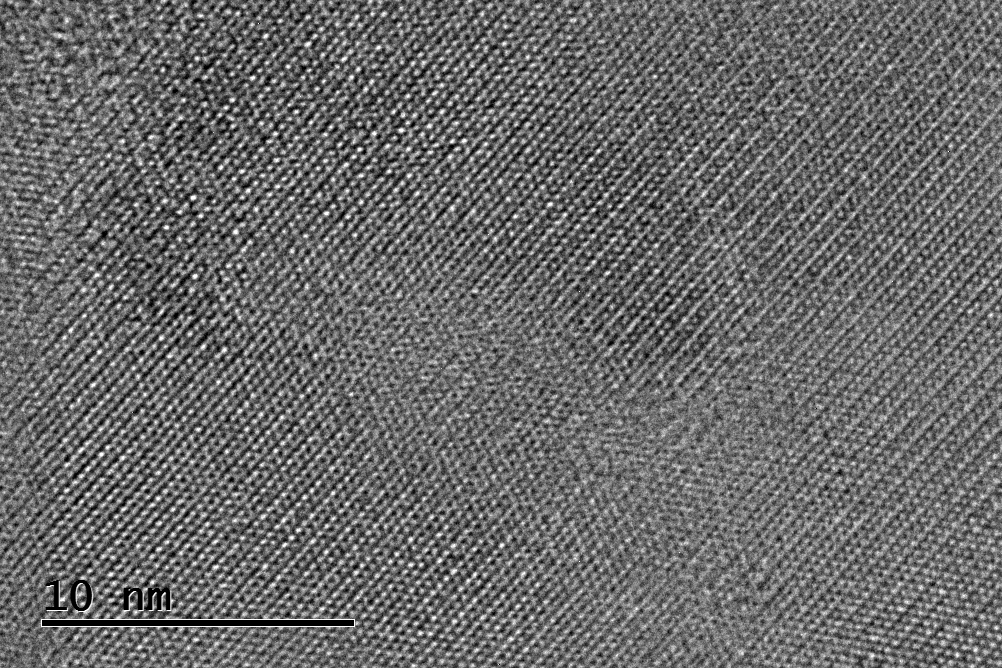
\includegraphics[width=\textwidth]{1T'/TEMImageHigh.png}
			\caption{High resolution TEM image.}
			\label{fig:1T'TEMImageHigh}
		\end{subfigure}
		\begin{subfigure}[b]{0.4\textwidth}
			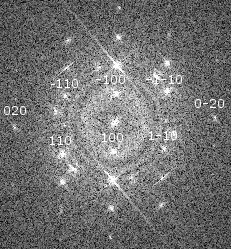
\includegraphics[width=\textwidth]{1T'/TEMEDFFT.png}
			\caption{FFT pattern constructed from the image in b).}
			\label{fig:1T'TEMEDFET}
		\end{subfigure}
		\caption{TEM characterisation of as grown 1T' flakes.}
		\label{fig:1T'TEMMaps}
	\end{center}
\end{figure}

In order to ascertain the phase of the as grown $WSe_2$ a Raman spectrum has been taken. As seen in Figure \ref{fig:1T'RamanSpectraComparison} the spectrum of the as grown 1T' $WSe_2$ looks very different to the Raman spectrum of the CVD grown 2H $WSe_2$ as seen in e.g. Figure \ref{fig:WSe2RamanSpectrum}. The $E^1_{2g}$ and $A_{1g}$ located around 250 $cm^{-1}$ and are convoluted in case of the monolayer. In spectrum of the 1T' sample (Figure \ref{fig:1T'RamanSpectraComparison}) the closest peaks to those are located at 248.6 and 260 $cm^{-1}$ and can be therefore ascribed to $E^1_{2g}$ and $A_{1g}$ modes respectively. Additionally the absence of the $B^1_{2g}$ peak suggest that the material is very thin. Furthermore there are 5 more unresolved peaks at 104.5, 149, 177, 218 and 236.3 $cm^{-1}$. Thus far there is no published information regarding the vibrational modes of 1T' $WSe_2$ and therefore the peaks cannot be assigned to the modes. Similarly new peaks have been reported for 1T' $MoS_2$ where new peaks were labelled as $J_1$, $J_2$ and $J_3$ \cite{Yu2018}.

\begin{figure}[!h]
	\begin{center}
		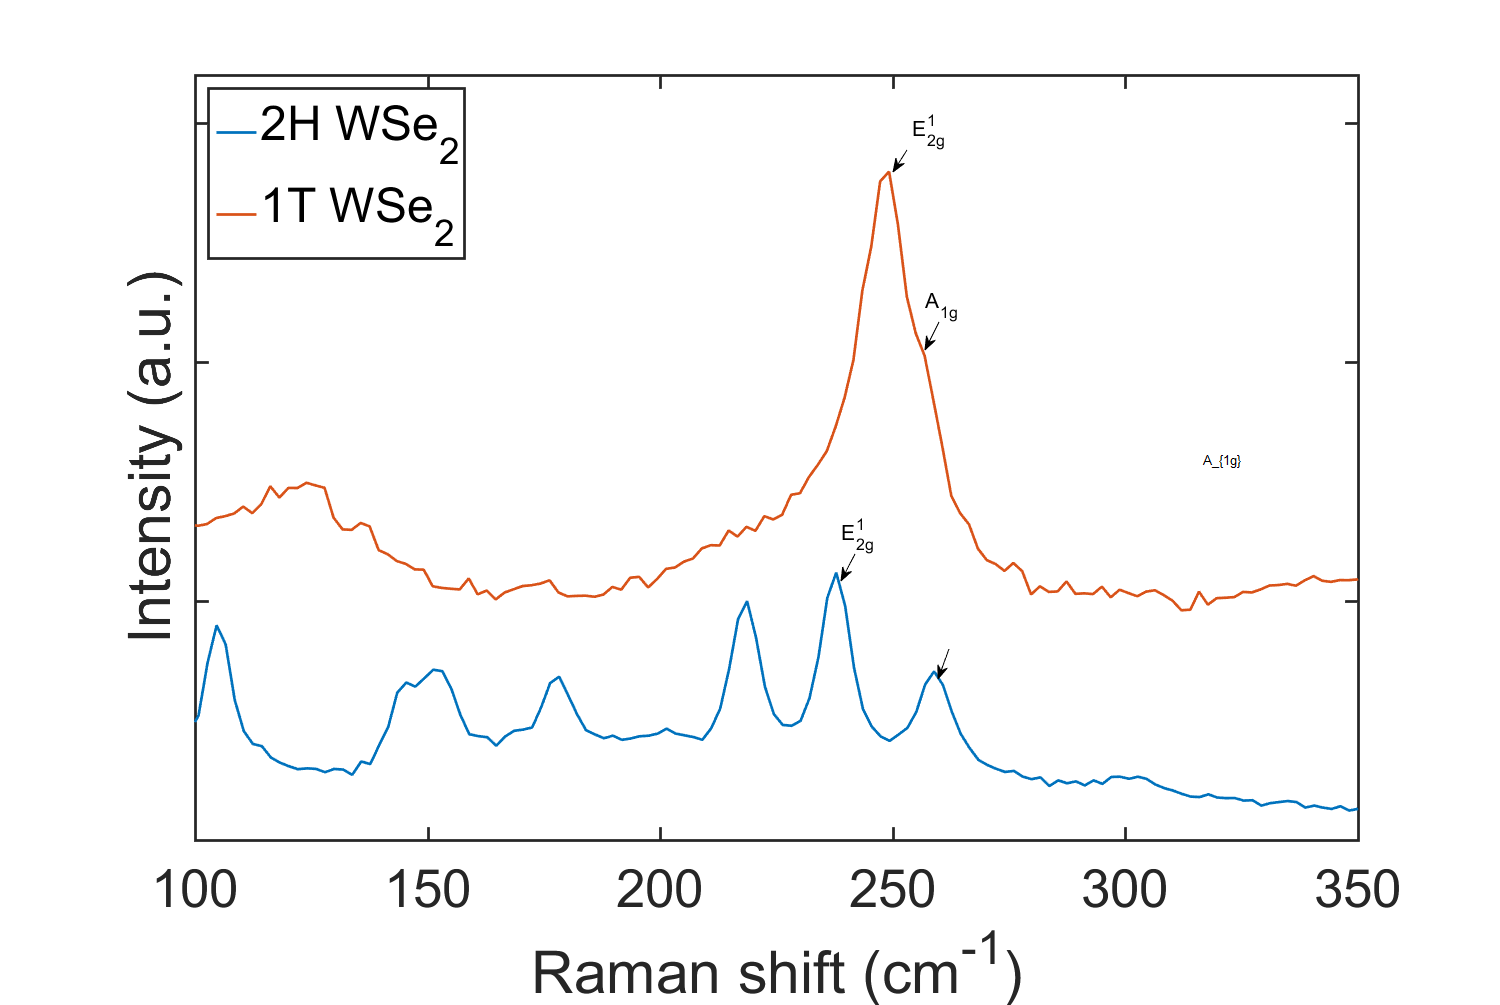
\includegraphics[scale=0.3]{1T'/RamanSpectraComparison.png}
		\caption{Raman spectra of 2H $WSe_2$ and 1T' $WSe_2$}
		\label{fig:1T'RamanSpectraComparison}
	\end{center}
\end{figure}

Similarly, the XPS spectra were taken of the as-grown sample as seen in Figure \ref{fig:1T'XPSW4fPreSpectrum} and Figure \ref{fig:1T'XPSSe3dPreSpectrum}. The XPS spectrum of the W 4f electron shell shows a doublet of $W^{+4}$ 4f at 31.49 and 33.63 eV. This position varies notably from those reported for 2H $WSe_2$ and therefore are attributed to 1T' $WSe_2$. The shift itself is most likely caused by change in coordination of the metal atom or a change in the W-Se bond length from 2.531 \r{A} to 2.66 \r{A}. On top of the 1T' phase of $WSe_2$ additional small contributions to the spectrum can be attributed to the 2H $WSe_2$ at 32.22 eV and 34.30 eV. Additionally an even smaller contribution from tungsten oxides can be identified at 35.74 eV and 37.92 eV. The Se 3d level spectrum seen in Figure \ref{fig:1T'XPSSe3dPreSpectrum} of the as-grown sample has been fitted with 4 doublets. Two of those doublets are associated with $Se^{-2}$ atoms and are assigned to 1T' $WSe_2$ (53.60 eV and 54.46 eV) and 2H $WSe_2$ (54.26 eV and 55.1 eV). The remaining two doublets, with much lower integrated area as compared to the Se bound to W, are assigned to amorphous Se (54.62 eV and 55.46 eV) and Se partially coordinated with phosphines (55.49 eV and 56.36 eV). The latter is remaining from the unreacted precursors of Se for the colloidal synthesis and a small component of amorphous Se is excepted as residual from the synthesis as well.

\begin{figure}[H]
	\begin{center}
		\begin{subfigure}[b]{0.7\textwidth}
			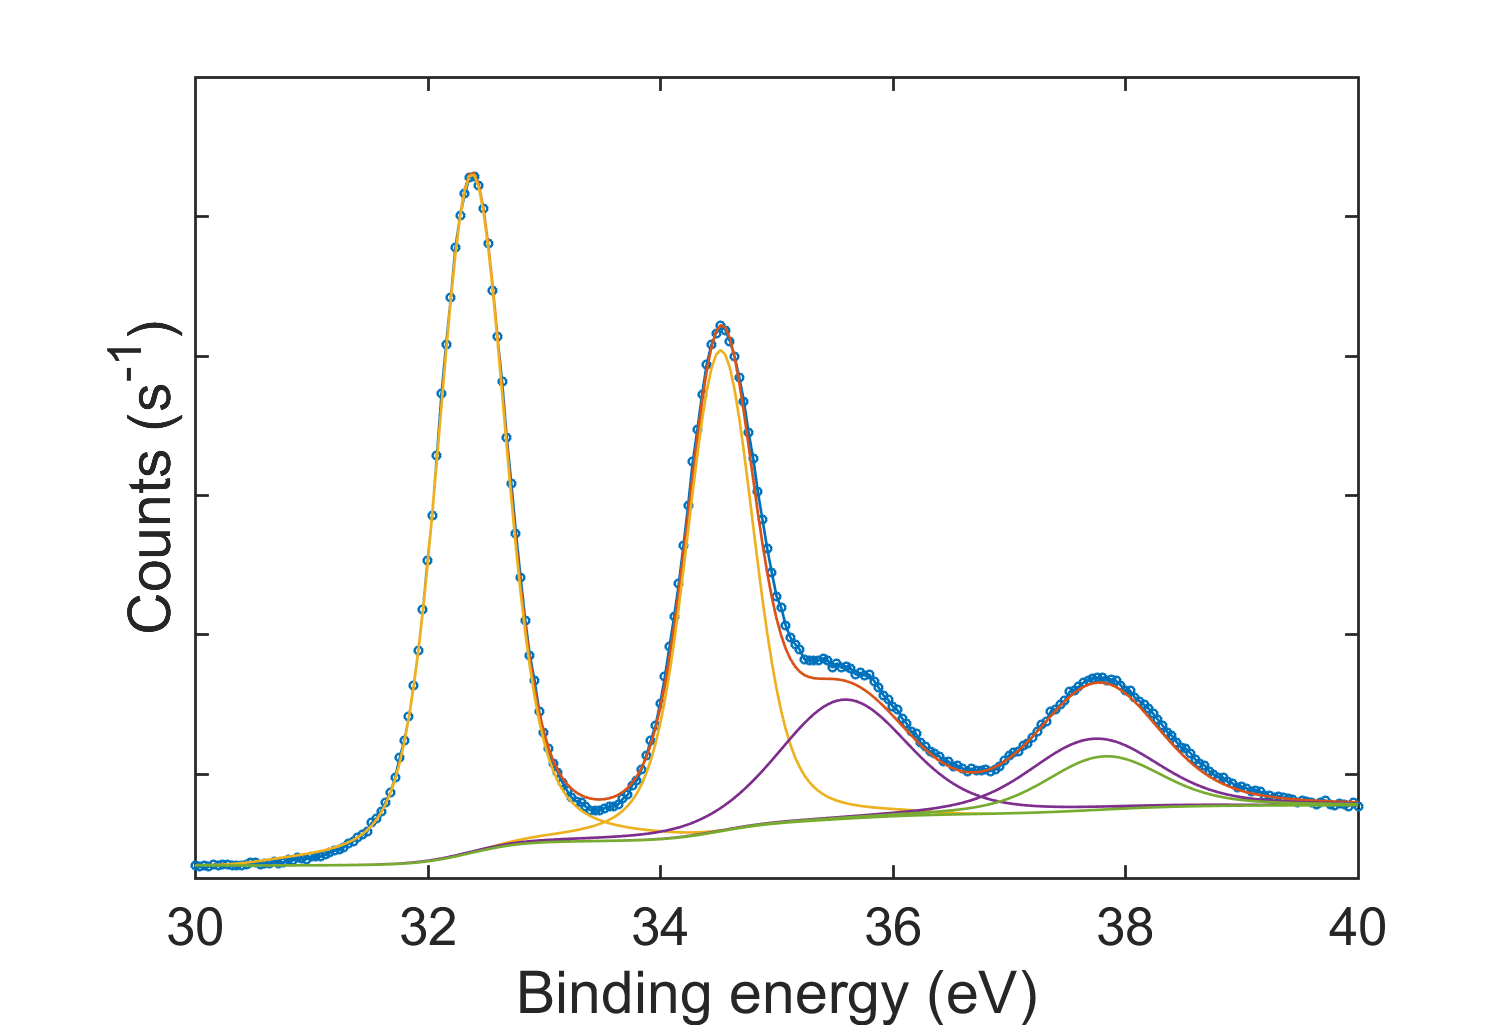
\includegraphics[width=\textwidth]{1T'/XPSW4fPre.png}
			\caption{W 4f}
			\label{fig:1T'XPSW4fPreSpectrum}
		\end{subfigure}
		\qquad
		\begin{subfigure}[b]{0.7\textwidth}
			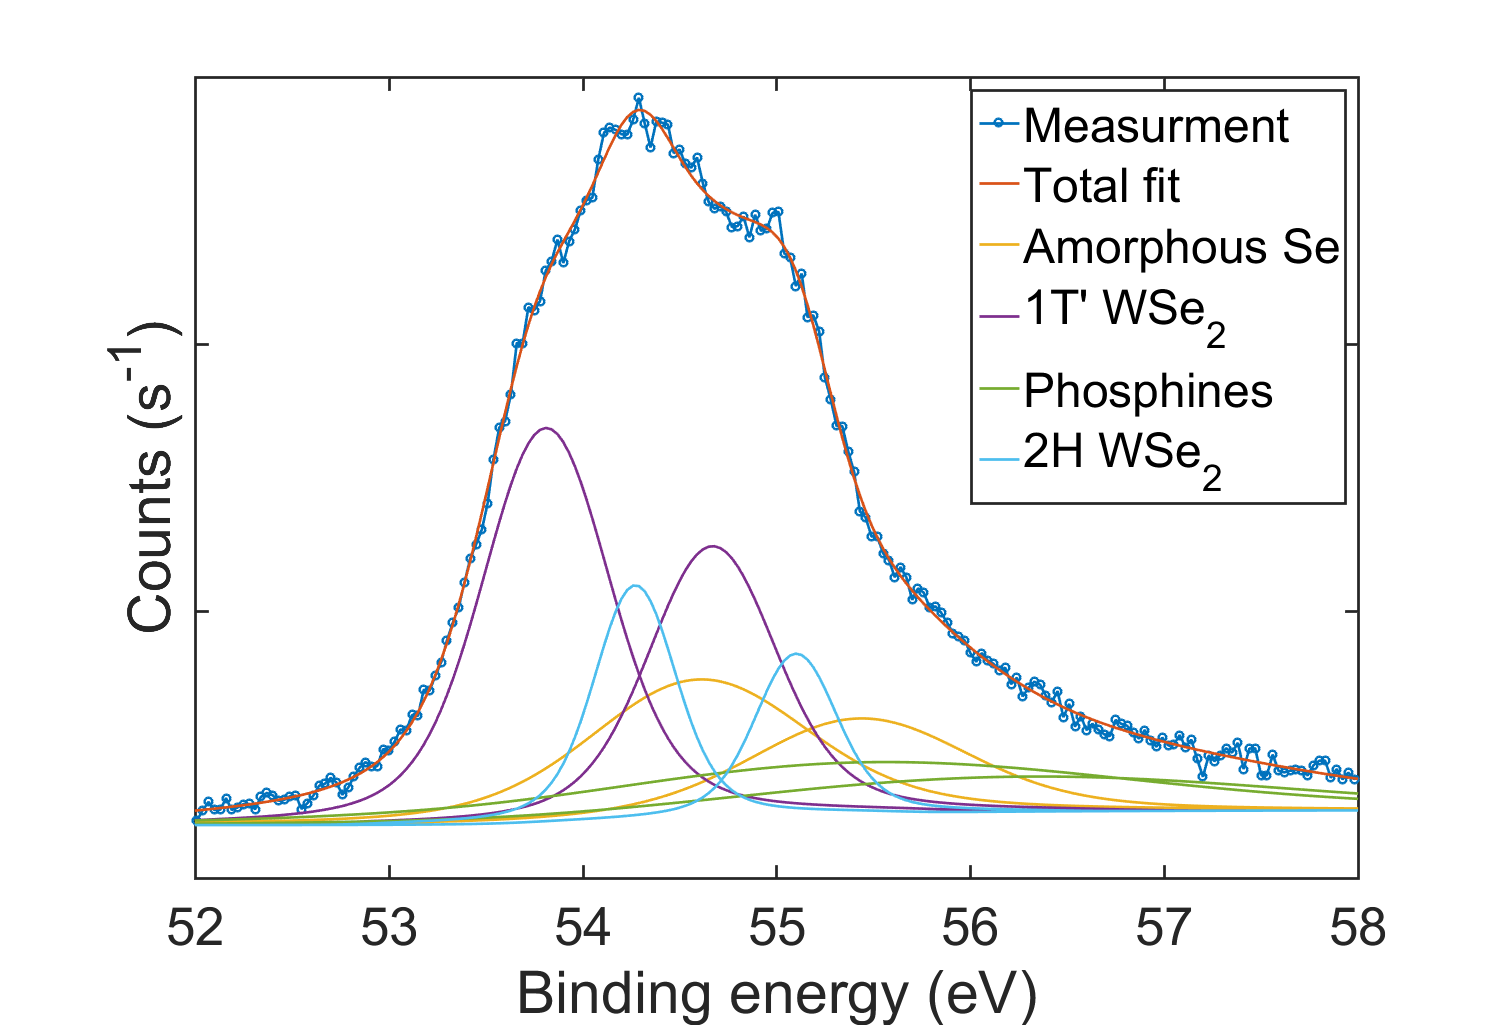
\includegraphics[width=\textwidth]{1T'/XPSSe3dPre.png}
			\caption{Se 3d}
			\label{fig:1T'XPSSe3dPreSpectrum}
		\end{subfigure}
		\caption{XPS spectra of W 4f and Se 3d levels in as grown sample of $WSe_2$}
		\label{fig:1T'XPSPreSpectra}
	\end{center}
\end{figure}

\begin{figure}[H]
	\begin{center}
		\begin{subfigure}[b]{0.7\textwidth}
			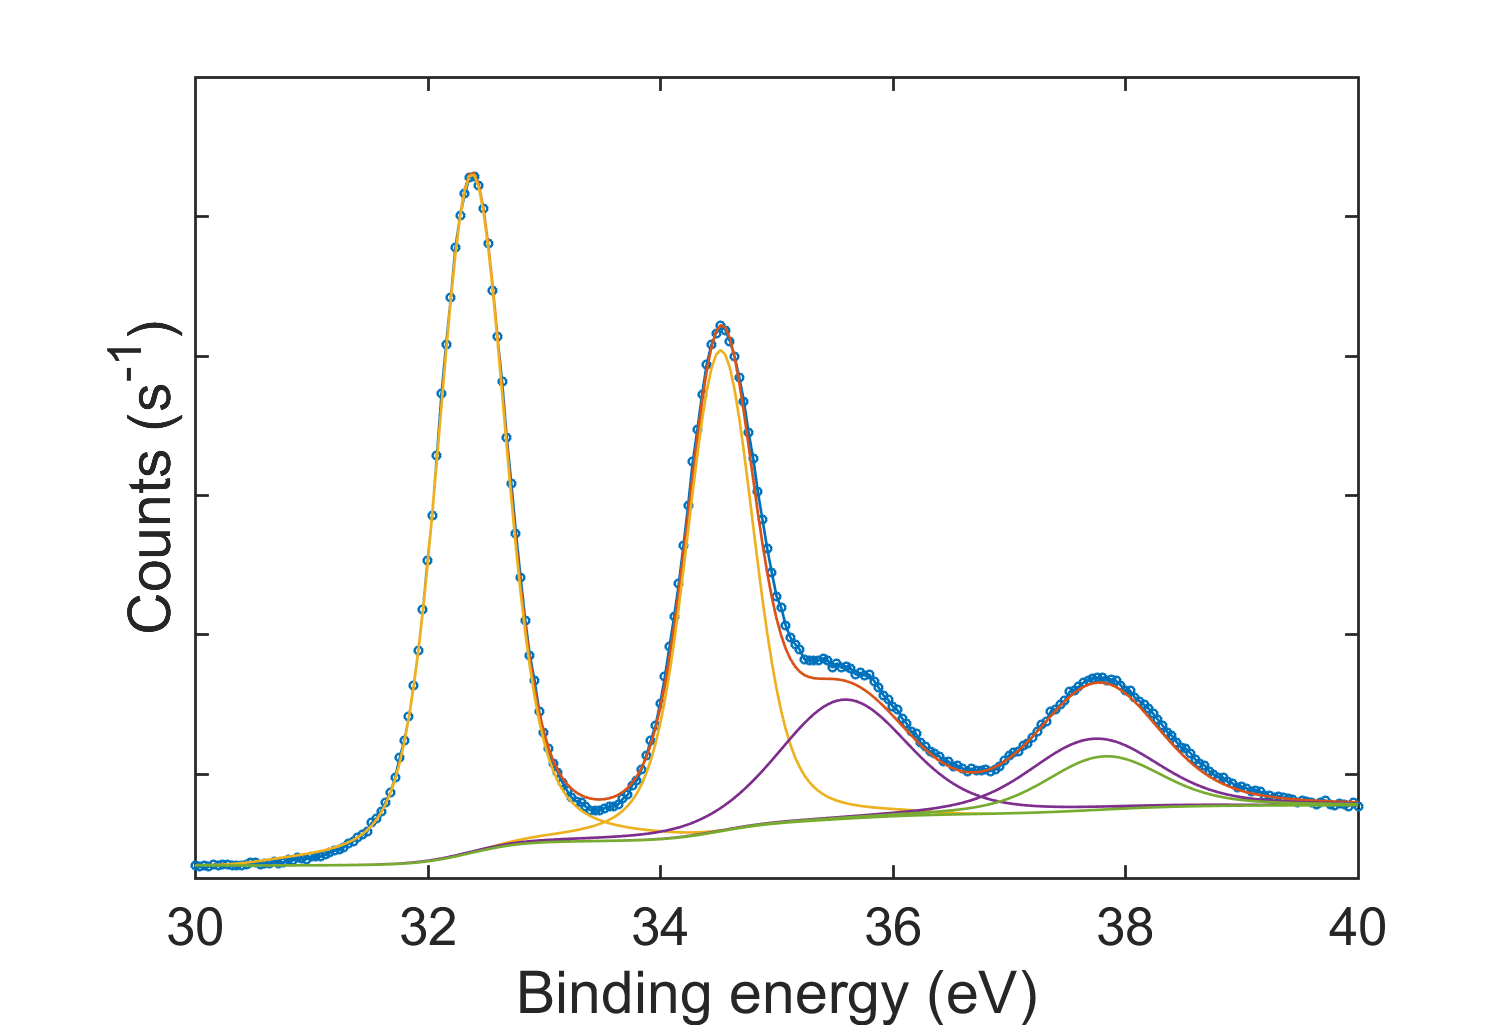
\includegraphics[width=\textwidth]{1T'/XPSW4fAnn.png}
			\caption{W 4f}
			\label{fig:1T'XPSW4fAnnSpectrum}
		\end{subfigure}
		\qquad
		\begin{subfigure}[b]{0.7\textwidth}
			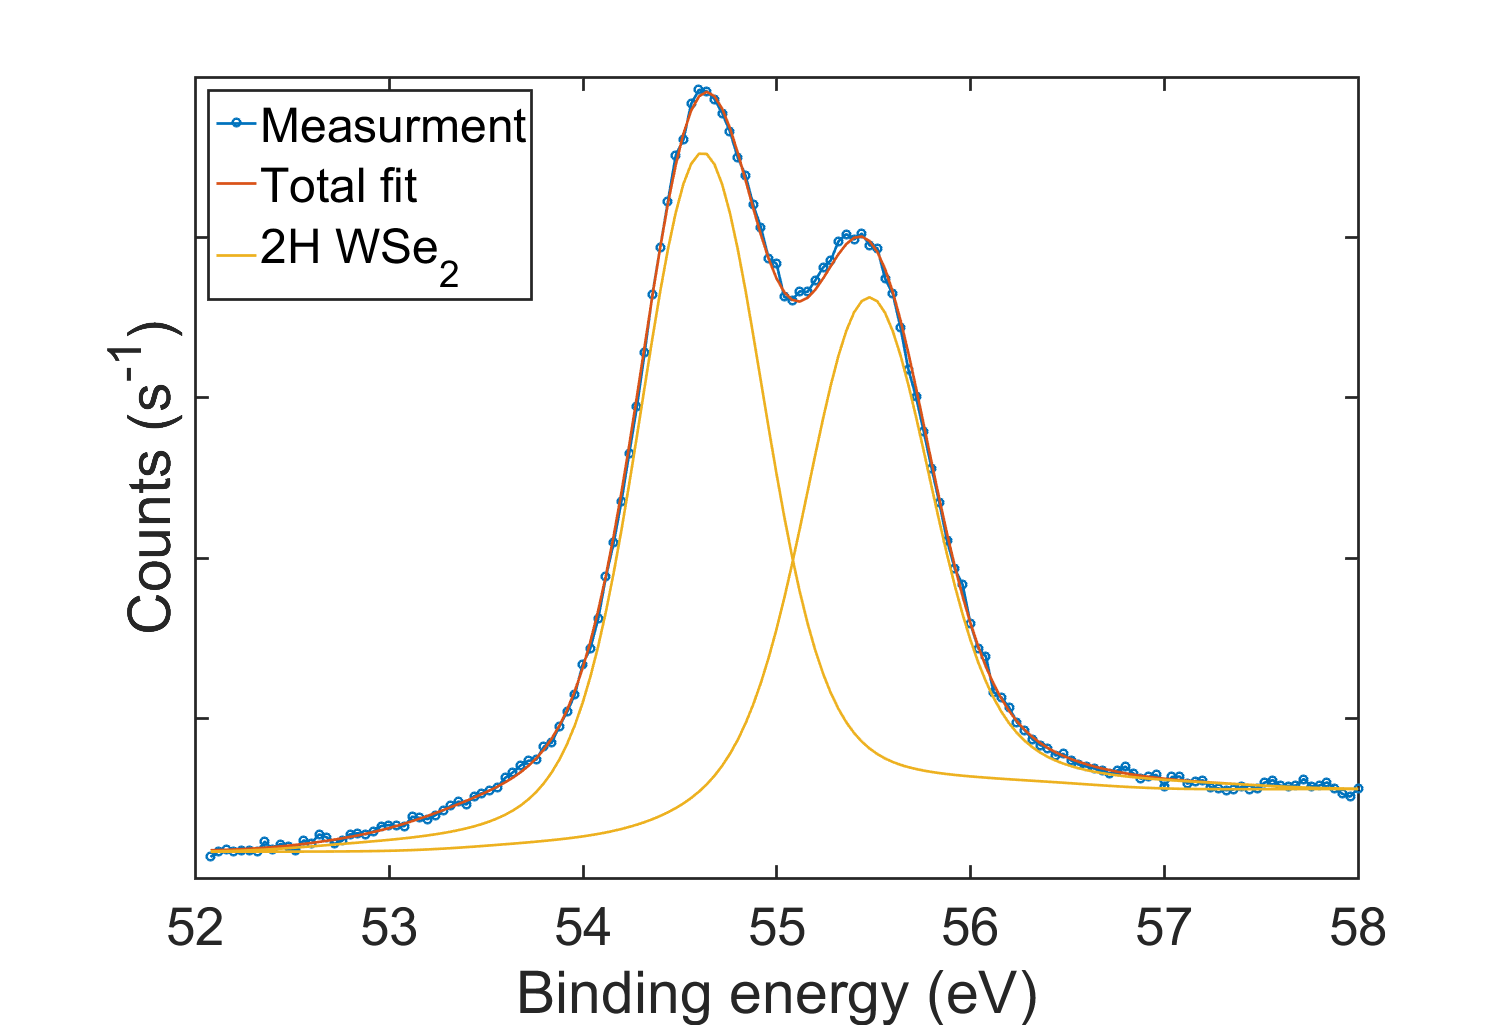
\includegraphics[width=\textwidth]{1T'/XPSSe3dAnn.png}
			\caption{Se 3d}
			\label{fig:1T'XPSSe3dAnnSpectrum}
		\end{subfigure}
		\caption{XPS spectra of W 4f and Se 3d levels in the annealed sample of $WSe_2$}
		\label{fig:1T'XPSAnnSpectra}
	\end{center}
\end{figure}

The as-grown sample was then annealed at 400 {\degree}C in an argon atmosphere. The Raman spectrum of the annealed sample can be seen in Figure \ref{fig:1T'RamanSpectraComparison}. The previously unidentified peaks are no longer present except for the two convoluted peaks at around 250 $cm^{-1}$. This is indicative of 2H $WSe_2$ and suggests that the entirety of the 1T' phase has been converted to the 2H phase. Additionally the XPS spectra of the annealed sample can be seen in Figure \ref{fig:1T'XPSAnnSpectra}. The presence of 4f $W^{4+}$ peaks 32.40 eV and 34.58 eV and an almost complete absence of the 1T' 4f $WSe_2$ indicates that the sample is primarily a 2H $WSe_2$. It is worth noting that after annealing the oxidized component of W just increases by a negligible amount. Following the annealing the XPS spectrum of the Se 3d can be seen in Figure \ref{fig:1T'XPSSe3dAnnSpectrum}. The spectrum can be fitted with one doublet associated with 2H $WSe_2$ only. This indicates that any residues of unreacted Se can be removed by annealing as expected as the evaporation temperature of elemental Se is $\sim$270 {\degree}C. 

\section{Conclusions}

In this chapter we have presented and discussed the electronic band structure and the physical characterization of CVD grown 2H $WSe_2$. The CVD synthesis of $WSe_2$ is quite challenging and not much work has been reported so far in the literature due to the low reactivity of Se. We have concluded that the grown material is pure, and possibly have high crystallinity as demonstrated from the relatively small FWHM of the PL peak. Additionally, thanks to micrometric lateral size resolution of the XPS analysis we could distinguish and parameterise the difference in binding energy of W 4f orbitals as a function of the thickness of the flakes for the first time. Furthermore, we could prove that a small amount of $WO_3$ is spread all over the substrate and it is not chemically bound to $WSe_2$. Similarly, it was interesting to observe the presence of elemental Se on the bare substrates. In contrast with the belief that the sticking coefficient of chalcogen elements is very low as compared to metals such as W and Mo, this evidence can shed light into the growth mechanism via CVD of atomically thin materials.

Additionally we have shown how the 1T' $WSe_2$ has been grown for the first time using this colloidal synthesis route. The material has then been characterised using Raman spectroscopy, XPS, TEM, and KPFM to ascertain to be in the 1T’ crystal phase and to demonstrate  to be metallic. Following an annealing at 400 {\degree}C the 1T' phase has been almost entirely converted to 2H. We have ascertain the presence of the 2H phase by preforming Raman spectroscopy, XPS, TEM, and characterization. This growth method therefore allows for direct deposition of metastable phase on a functional substrate. Our Raman and XPS characterization of the 1T’ phase represent a reference in the literature for future synthesis of 1T’ phases of TMDCs.